\documentclass{article}

\usepackage{blindtext}
\usepackage{titlesec}
\usepackage{graphicx}
\usepackage{fancyhdr}
\usepackage{caption}
\usepackage{listings}
\usepackage{color}
\usepackage{indentfirst}
\usepackage[hyphens]{url}
\usepackage[hidelinks]{hyperref}

\graphicspath{ {./images/} }

\definecolor{dkgreen}{rgb}{0,0.6,0}
\definecolor{gray}{rgb}{0.5,0.5,0.5}
\definecolor{mauve}{rgb}{0.58,0,0.82}

\newcommand{\subsubsubsection}[1]{\paragraph{#1}\mbox{}\\}
\setcounter{secnumdepth}{4}
\setcounter{tocdepth}{4}

\usepackage[a4paper, total={6in, 8in}]{geometry}
\setlength{\parskip}{0.8em}

\title{CM3070 Final Project - Preliminary Report}
\author{Esteban Garcia}
\date{ }
\pagestyle{fancy}
\fancyhf{}
\lhead{CM3070 Final Project - Preliminary Report}
\rfoot{Page \thepage}

\begin{document}
  \maketitle

  \tableofcontents

  \newpage
  \section{Introduction}

  For my project I'm going to be using the non-profit web application template.

  In the modern era of software development, the rapid adoption of third-party open-source libraries and containerised applications has revolutionised how software is built, deployed, and maintained. This shift has brought significant improvements on how we build software. However, it has also introduced new security challenges. As today's software supply chain increasingly depends on external dependencies, the potential attack surface for malicious actors has expanded dramatically.

  Software supply chain security aims to address the risks associated with this by ensuring that the integrity, provenance, and authenticity of software artifacts are safeguarded. High-profile supply chain attacks, such as SolarWinds and the exploitation of vulnerabilities like Log4Shell, underscore the critical need to secure software delivery and have demonstrated how a single compromised artifact can cascade through an ecosystem, affecting millions of users and causing substantial damage.

  To mitigate such risks, organisations and communities are adopting artifact management tools that enforce stricter security standards. These tools centralise the third-party dependencies and allow organisations to verify their origins, cryptographically sign artifacts and block software with known vulnerabilities.

  The Open Container Initiative (OCI) [1] compliance plays a pivotal role in this effort, as it promotes interoperability and consistency in how software can be packaged, distributed, and executed.

  OCI is a set of open-source standards designed to create a unified framework for container technology, focusing on interoperability and consistency across different container platforms.

  These standards were developed mostly with container technology (docker) in mind but starting with the OCI v1.1 specification, now it can be used to store any type of artifact as long as the specs are followed.

  Making it suitable to support different artifact formats beyond just Container Images, bringing then the benefits of the OCI standard to them.

  Motivated by these considerations, my project aims to provide a secure platform for storing, managing, and distributing OCI artifacts.

  Using OCI as a storage layer allows for my project to leverage its capabilities to store any kind of software, this reduces compatibility issues and fosters consistency in development and deployment environments. 

  It ensures that artifacts are verifiable and tamper-proof through tools like digital signatures and hash-based verification.

  OCI-compliant tools integrate seamlessly with various ecosystem tools, such as container registries, Kubernetes, and CI/CD platforms. This interoperability makes it easier to share, store, and retrieve artifacts across diverse environments

  By following these standards, artifacts become more portable and adaptable, allowing organizations to easily move and deploy artifacts across cloud environments, on-premise systems, or hybrid infrastructures

  As there is a wide selection of different package formats in the ecosystem to prevent scope creep I will focus only on storage and distribution of Docker Images [2], Helm Charts [3] and PyPi Packages [4]. This last one is the only format that doesn't support the OCI protocol so a translation layer would need to be developed but it will serve as proof of the standard's capabilities to store and distribute any type of software.

  \section{Literature Review}

  \subsection{Similar Projects}

  This section provides an analysis of existing solutions, the two projects I'm focusing in here are JFrog Artifactory [5] and Harbor [6]. These platforms have two different approaches to artifact management and container registry functionality.
  
  JFrog Artifactory as a commercial, enterprise-grade solution with extensive support for different artifact formats, and Harbor as an open-source OCI compliant registry.

  This analysis will provide a foundation for understanding the design and implementation decisions behind the project, demonstrating how it aims to bridge existing gaps and contribute to the evolution of secure artifact management practices.

  \subsubsection{JFrog Artifactory (commercial product)}

  JFrog Artifactory is a commercial, universal artifact repository manager. It supports a wide range of package formats (e.g., Docker images, Maven, npm, PyPI) and integrates into CI/CD pipelines. It is well-known for its scalability, enterprise-grade features, and extensive integrations.

  The product offers no free version and is offered with both a cloud and a self-hosted solution. Its cloud-based product is not multi-tenant, meaning that JFrog needs to deploy standalone infrastructure for each customer, and its self-hosted solution is deployed and managed by the customer.
  
  Due to its closed-source nature, and lack of multi-tenancy features, this means that organisations can't be aware of any security vulnerabilities in the platform and patching of these would require JFrog to implement the fix, notify their self-hosted customers and then apply the patch to each Cloud instance administered by them.

  This last point is concerning as reported by Google in their latest report [7] we've been seeing the Time-To-Exploit metric being reduced from 32 days in 2021 \& 2022 to 5 days in 2023, and 97\% of them being exploited as zero-days vulnerabilities.

  Artifactory classifies itself as an `universal' artifact management platform, meaning it provides the capabilities to store any type of package format and new ones are being implemented all the time. But it uses its own Storage Architecture Layer and API that doesn't adhere to any open-source standard.

  Artifactory is OCI-compliant but the standard is not used as the storage layer for all of its supported format but rather only for OCI-artifacts only. 

  So this means that custom JFrog-developed libraries have to be used to interface with its APIs for administering artifacts outside of each format's native tooling.

  JFrog uses their own close-sourced static analysis vulnerability scanner called XRay [8], as it's a separate product it needs to be payed separately.

  At the same time signature [9] of uploaded packages is an `enterprise' only feature.

  Artifactory is a very complete solution but only accesible to those with a big budget and requires a lot of administrative effort to create a secure supply chain for an organization's software.
  
  \subsubsection{Harbor (open-source project)}

  Harbor is an open-source container image registry, built by VMware [10] and now part of the Cloud Native Computing Foundation [11]. It is designed to enhance container image security and improve efficiency in managing containerized environments.

  As it's an open-source project, Harbor benefits from community-driven development and transparency.

  In contrast to Artifactory, Harbor is fully self-hosted and requires the operator to deploy and administer its infrastructure without an multi-tenant cloud-hosted option.

  It's an fully OCI-compliant registry, this enables seamless integration with OCI-complaint tooling allowing developers/devops engineers to manage artifacts with either Harbor's Custom Tooling or native OCI tools. It only supports the upload of OCI artifacts, package formats that don't adhere to the standard can't be uploaded without additional custom automation.

  It provides vulnerability scanning by connecting to Trivy [12] or Clair [13], two open-source static analysis tools, these tools have to be deployed separately by the administrator.

  \subsubsection{Conclusion}

  Both projects have extensive support and can be used to secure an organisation's software supply chain.
  Even though Artifactory is OCI-compliant its underlying storage architecture is not based on that technology, increasing the complexity for its users and its commercial nature limits its usage only to those with deep enough pockets to pay for it.

  Harbor is fully OCI-compliant and open-source, it benefits from its transparency with the community but it focuses only on OCI/Container artifacts, doesn't support other package formats so it can't be used as a full solution to secure the supply chain.

  \subsection{Research Studies}

  In this section I evaluate different reserach studies that justify the development and usage of a project like the one I'm developing.
  
  William Enck and Laurie Williams define the Three of the Top Five Challenges in Software Supply Chain Security [14] as:

  \begin{itemize}
    \item updating vulnerable dependencies
    \item choosing trusted supply chain dependencies
    \item securing the build process
  \end{itemize}

  For a developer to be able to secure their software, they need to be aware of vulnerabilities on their dependencies, this process has to be automated so a platform that is aware of a software's dependencies has to be used for this.

  Choosing trusted supply chain dependencies is very important, what if a library your software is dependent on is deleted and someone takes the name? You don't only need to establish trust with the dependency you are using but also with the Package Index is coming from, most of the programming languages out there have some kind of public package index, PyPi for Python, NPM for NodeJS, there's good intentention behind these services but there's no guarantee that anything being uploaded there is safe as there is no vetting nor barrier to entry.

  Package Typo-squatting, a form of social-engineering attack that targets users who incorrectly type a package's name, is becoming more normal in public package indexes, a good example discovered by a member of the Python community named Bertus [15] who reviewed a malicious package named `pytz3-dev' seen in the Python package index (PyPi). This package targeted developers looking for the very popular `pytz' package, it executed malicious code that searched for a SQLite database used by Discord the popular chat application, this database is used by Discord to store user information locally but also it includes tokens used to authenticate the user against the service.

  So a developer should upload their dependencies to a trusted store where they have control over what goes in and what goes out.

  Recently the NSA released a paper on recommended practices for developers on how to secure the software supply chain [16], as part of their recommended Secure Development Practices, they recommend that all third-party libraries are uploaded to a secure repository where they can be analysed for vulnerabilities on an on-going basis and an audit log of upload and downloads of libraries is kept.
  
  \subsection{OCI v1.1 Distribution Specification}

  Before I can start defining the design for my project there needs to be an understanding of the OCI v1.1 Distribution Specification [17]. I'm going to explain the basic functionality needed for my project to be conformant with the specification, without going into too much detail as the document referred is a better source for it.

  This specification defines the API protocol to facilitiate and standardize the distribution of OCI artifacts, and it is design to be agnostic of content type. Container Images is the most prominent type but the protocol is open to any.

  There are four different types of workflows as part of the specification:

  \begin{itemize}
    \item Pull - Clients are able to pull from the registry
    \item Push - Clients are able to push to the registry
    \item Content Discovery - Clients are able to list or otherwise query the content stored in the registry
    \item Content Management - Clients are able to control the full life-cycle of the content stored in the registry
  \end{itemize}
  
  \subsubsection{Terms Definitions}

  Before going in detail into the different categories, there are certain terms that warrant basic definitions:

  \begin{itemize}
    \item Repository: a scope for API calls on a registry for a collection of content (including manifests, blobs, and tags).
    \item Blob: the binary form of content that is stored by a registry, addressable by a digest
    \item Digest: a unique identifier created from a cryptographic hash of a Blob's content, normally SHA-256
    \item Manifest: A JSON document uploaded to the registry, it serves as an index, providing information needed to retrieve and assemble the layers and configurations that make up an artifact.
    \item Layers: A list of descriptors for the artifact, each pointing to a specific uploaded blob
    \item Push: the act of uploading blobs and manifests to a registry
    \item Pull: the act of downloading blobs and manifests from a registry    
    \item Tag: a custom, human-readable pointer to a manifest. A manifest digest may have zero, one, or many tags referencing it.
  \end{itemize}
  
  \subsubsection{Pull}

  This is the process of pulling manifest and blobs from the registry and typically the first step in pulling an artifact is to retrieve its manifest as it contains all the information on what blobs need to be downloaded.

  \subsubsubsection{Pulling manifests}
  
  This is done by performing a `GET' request to the registry to the URL \url{/v2/<name>/manifests/<reference>}

  Where `name' is the name of the repository and `reference' either the digest of the manifest or a tag.

  \subsubsubsection{Pulling blobs}

  This is done by performing a `GET' request to the registry to the URL \url{/v2/<name>/blobs/<digest>}

  Where `name' is the name of the repository and `digest' is the blob's digest

  \subsubsubsection{Checking for content existance}

  To verify for the existance of either a blob or a manifest a `HEAD' request to either the pull manifest or blobs URLs. A successful response would indicate that the content exists in the registry.

  \subsubsection{Push}

  This is the process of pushing manifests and blobs to the registry, and it works in the opposite order described previously, blobs are pushed first and the manifest last.

  \subsubsubsection{Pushing blobs}

  There are two ways to push blobs: chunked or monolithic. A monolithic upload happens as a single request to the registry, a chunked one consists of multiple upload request each one with a chunk of the blob. Each chunk is uploaded in order from start to finish.
  
  The client decides which type of push mechanism wants to use, but as a general rule of thumb, monolithic pushes will be used to upload small blobs and chunked to upload very big ones.

  There are two ways to push a blob monolithically, a POST request followed by a PUT request [18] or a single POST request [19].
  
  Chunk uploads are similar to the first option for a monolithic upload, the first POST request starts an upload session, then multiple PUT requests are made to the registry each one with a chunk of the blob, afterwards the upload is finalised by a last PUT request that also includes the cryptographic hash of the blob, this signals to the registry that the upload session is finished.
  
  \subsubsubsection{Pushing manifests}

  To push a manifest a PUT request to the following URL is performed: \url{/v2/<name>/manifests/<reference>}

  Where `name' is the name of the repository and `reference' either the digest of the manifest or a tag.

  A manifest can have a different `Content-Type' depending on the type of artifact being pushed and it is used to identify the type of artifact server-side.
  
  Example `application/vnd.oci.image.manifest.v1+json' determines that the pushed manifest is for a OCI Container Image.

  This will be leveraged to identify what type of artifact we are receiving and also to create our own custom artifacts for those package formats that aren't supported out of the box by OCI.

  The request contains the cryptographic hash of the manifest used to reference it and it can optionally contain a tag too.

  \subsubsection{Content Discovery}

  These set of endpoints are used to fetch information from the registry about available artifacts.

  \subsubsubsection{Listing Tags}

  To fetch the list of tags a GET request to the following URL is performed: \url{/v2/<name>/tags/list}

  Where `name' is the name of the repository. The registry has to returned all available tags for the specified repository.

  \subsubsubsection{Listing Referrers}

  This is a new endpoint released as part of the OCI v1.1 specification [20]. A manifest can refer to a different manifest creating a relationship between the two, this endpoint allows for fetching all related artifacts for a specific manifest.
  
  This is good to attach things like signatures to an OCI artifact.

  To fetch the list of referrers a GET request to the URL is performed: \url{/v2/<name>/referrers/<digest>}

  Where `name' is the name of the repository, and `digest' is the digest of the manifest.

  Upon success, the response must be a JSON body with an image index containing a list of descriptors

  \subsubsection{Content Management}

  Content management refers to the deletion of blobs, tags, and manifests. These are optional endpoints that a registry may implement.

  \subsubsection{Authentication}
  
  The specification defines that registries may require authentication to interact with the registry.

  For this registries needs to return an `401 Unauthorized' error, including a `WWW-Authenticate' header with the URL for the login challenge and the Authentication scheme.
  
  The client then needs to send base64 encoded, basic authentication credentials to the endpoint and on successful response it will recieve back a token comformant with the authenciation scheme provided. 

  \section{Design}

  My project, operates in the domain of software artifact management, focusing on creation, storage, management, and distribution of software artifacts, which are essential components of modern DevOps workflows.

  \subsection{Primary Users and Interaction interfaces}

  The primary users of my project include:

  \begin{itemize}
    \item Software developers
    \item DevOps Engineers and Site Reliability Engineers
    \item Security Teams
  \end{itemize}
  
  Therefore the design of it will focus on making it usable for them, most of the time these kind of users don't use UIs very often but rather CLI tooling that integrates with the programming languages or artifact types they use.

  Due to this, this will be the most important ways of interaction:

  \begin{itemize}
    \item OCI-compatible APIs
    \item Native OCI-compatible tooling, like Docker, ORAS (OCI Registry As Storage) [21], Helm
    \item Twine [22], a CLI tool for uploading Python Wheels to PyPi-compatible indexes and pip the Python package installer
  \end{itemize}

  A web UI will also be provided for administrative tasks outside the previously mentioned tooling.

  \subsection{Authentication}

  Security is an key aspect here, so we need to have strong access control to only allow uploads or downloads of artifacts to users that are authenticated and have the right permissions.

  The project will be secured using the Bearer authentication scheme [23]. All users will need an valid JWT Token [24] to successfully authenticate against the API.

  To avoid storing sensitive credentials that could be leaked in the case of a data breach, I will instead be leveraging AWS Cognito [25] an OAuth2 provider [26], with this I don't need to store sensitive credential data and can just verify incoming if an incoming JWT token was issued by my AWS Cognito User Pool.

  This means that signup and, by default, authentication happen outside the control of the application too. This is fine for the Web UI but for OCI-compliant tooling we need to provide a login endpoint, receive the user's credentials and exchange them for a JWT token. Luckily OAuth2 has a flow designed for this called the username-password flow [27] and Cognito supports it, so I will be leveraging this functionality for credentials exchange on the OCI login endpoint. The usage of this authentication flow is discourage as it means the application has to recieve user credentials directly, but unfortunately for now most OCI-tooling doesn't have support for OAuth2-compatible authentication mechanisms.

  The application would still need to at least be aware of user signups and maintain a User profile to be used for RBAC authorization, as signup and signin occur completly outside the control of the application I will be leveraging Cognito Triggers to execute an AWS Lambda function that will send a message to an SQS queue, a background worker will consume these messages and create an entry on the database.

  \subsection{Access Control}

  With authentication sorted, the project has to deny access to an authenticated user to resources it doesn't have the necessary permissions for.

  To be able to do this I need to define some virtual segmentation units that a user has to belong to or have access to, to be able to interact with the resources within them.

  As mentioned in my literature review, the analysed projects lack multi-tenancy, this will be a feature in my project and it will allow for virtual segmentation of organisations.

  Segmentation unit definition:
  \begin{itemize}
    \item Organisation: These represent administrative units within the project, serving as access control boundaries. Users must be members of an organisation to view, manage, or interact with the resources it contains.
    \item Registries: These are virtual segmentation units within an organisations and are where an OCI artifacts are stored. They provide a logical namespace for organizing and managing artifacts.
  \end{itemize}

  I plan on leveraging an RBAC architecture to control an user's access to resources within the application. A user could have any of these three roles within an organisation:
  \begin{itemize}
    \item Viewer: A user with viewer role will only have read-only access to the resources to the organisation it belongs to. This means it will only be able to list registires and artifacts and pull them.
    \item Writer: A user with the writer role has all the permissions of the viewer role, plus it can push and delete artifacts
    \item Admin: A user with full administrative control of all resources within the organisation, it has all the permissions of the writer role and it can manage members of the organisation.
  \end{itemize}

  \subsection{Artifact Storage}

  As the backbone of the project is storing Artifact Blobs and their availability for my users is the most important aspect of the project, I will be leveraging the AWS Simple Storage Service (S3) [27] as my base storage layer.

  S3 is a highly scalable and durable object storage service by AWS, it has 99.999999999\% durability and 99.99\% availability [28], it also has features like encryption, lifecycle management and object versioning making it a perfect solution for storing OCI artifacts in a safe manner.

  As S3 has a really powerful API to query for files, I'm also going to be leveraging these capabilities to know if a blob exists or not without having to store this data in the application's database.

  Both uploaded Blobs and Manifests will be stored on an S3 bucket. Given the nature of how OCI uploads work, there will be a 2-tier approach to storing them.

  As explain in the OCI section of the literature review, the upload of a blob works in the following way:

  \begin{enumerate}
    \item An upload session is initiated for a specific OCI artifact in a repository.
    \item The blob data is uploaded
    \item The upload is finished and the client sends the blob digest
  \end{enumerate}

  We receive the full data of the blob before knowing its digest, and given the content addressable storage of OCI the application has to store the blob alongside its digest on S3 to be able to address it, so to circumvent this the application will do the following:

  \begin{itemize}
    \item When an upload session is requested by the client, a random ID will be generated.
    \item In-flight blobs, these will be blobs that we received but don't know the digest yet, will be stored in S3 under a key called `in-flight'
    \item Once the upload session is finished and the application receives the digest for the blob, it will leverage the S3 API to move the file to the final location using the digest as key.
  \end{itemize}

  As S3 has a limit for a single file upload of 5 GB, OCI artifacts, specially container images can very quickly reach that limit. So to account for this the multipart upload API [29] will have to be used, with this objects up to 5TB can be uploaded. The way the application will manage this is by creating an multipart upload session when an OCI client requests a new upload session and finalise it when the OCI upload session is finalised too.

  With the data stored on S3, I can then create self-expiring presigned[30] links and redirect the user directy to S3 to download a blob or manifest without having to keep a connection to my own application, reducing load and making it more cost-effective to run.

  \subsection{Implementing the PyPi interface}

  As mentioned before my project is based on the OCI protocol, but as I would like to expand its functionality to also support the PyPi index repository interface to store and serve python packages.

  As PIP is not an OCI-compatible package manager, I need to implement an server-side interface to translate from the OCI protocol to the expected PyPi index responses.

  There are two endpoints that need to be created for this.

  \subsubsection{Upload API}

  The PyPi Upload API [31] endoint is the endpoint that tools such as Twine use to upload packages to PyPi. 

  My project would need to support this endpoint. This is a POST request to the `/legacy' URL, and it recieves a `.whl' file.

  To interface with OCI, this endpoint would need to receieve the file, upload it as a blob and create a manifest that refers the blob with a custom `mediaType'.

  A tag equivalent to the package's version that referrs to the created manifest's digest will be created.
  
  This will automatically expose the Python package via the OCI APIs. But for pip to be able to discover this package the application needs to implement the Simple Index Repository API endpoint.

  \subsubsection{Simple Repository API}

  The Simple Repository API is a set of two endpoints used by PIP to discover packages in a Python Repository.

  This is based on the PEP-503[32] and PEP-691[33] specifications.

  The endpoint returns all available Python packages in the repository or all available versions for a specified package.

  The output of this is either HTML or JSON depending on the `Content-Type' requested by the client.

  To implement this in my project, the endpoint would need to discover all OCI artifacts with the custom `mediaType' created on upload and dinamically generate the HTML or JSON response, this will allow for PIP to download Python packages stored on an OCI-compliant repository.

  \subsection{Architecture Diagram}

  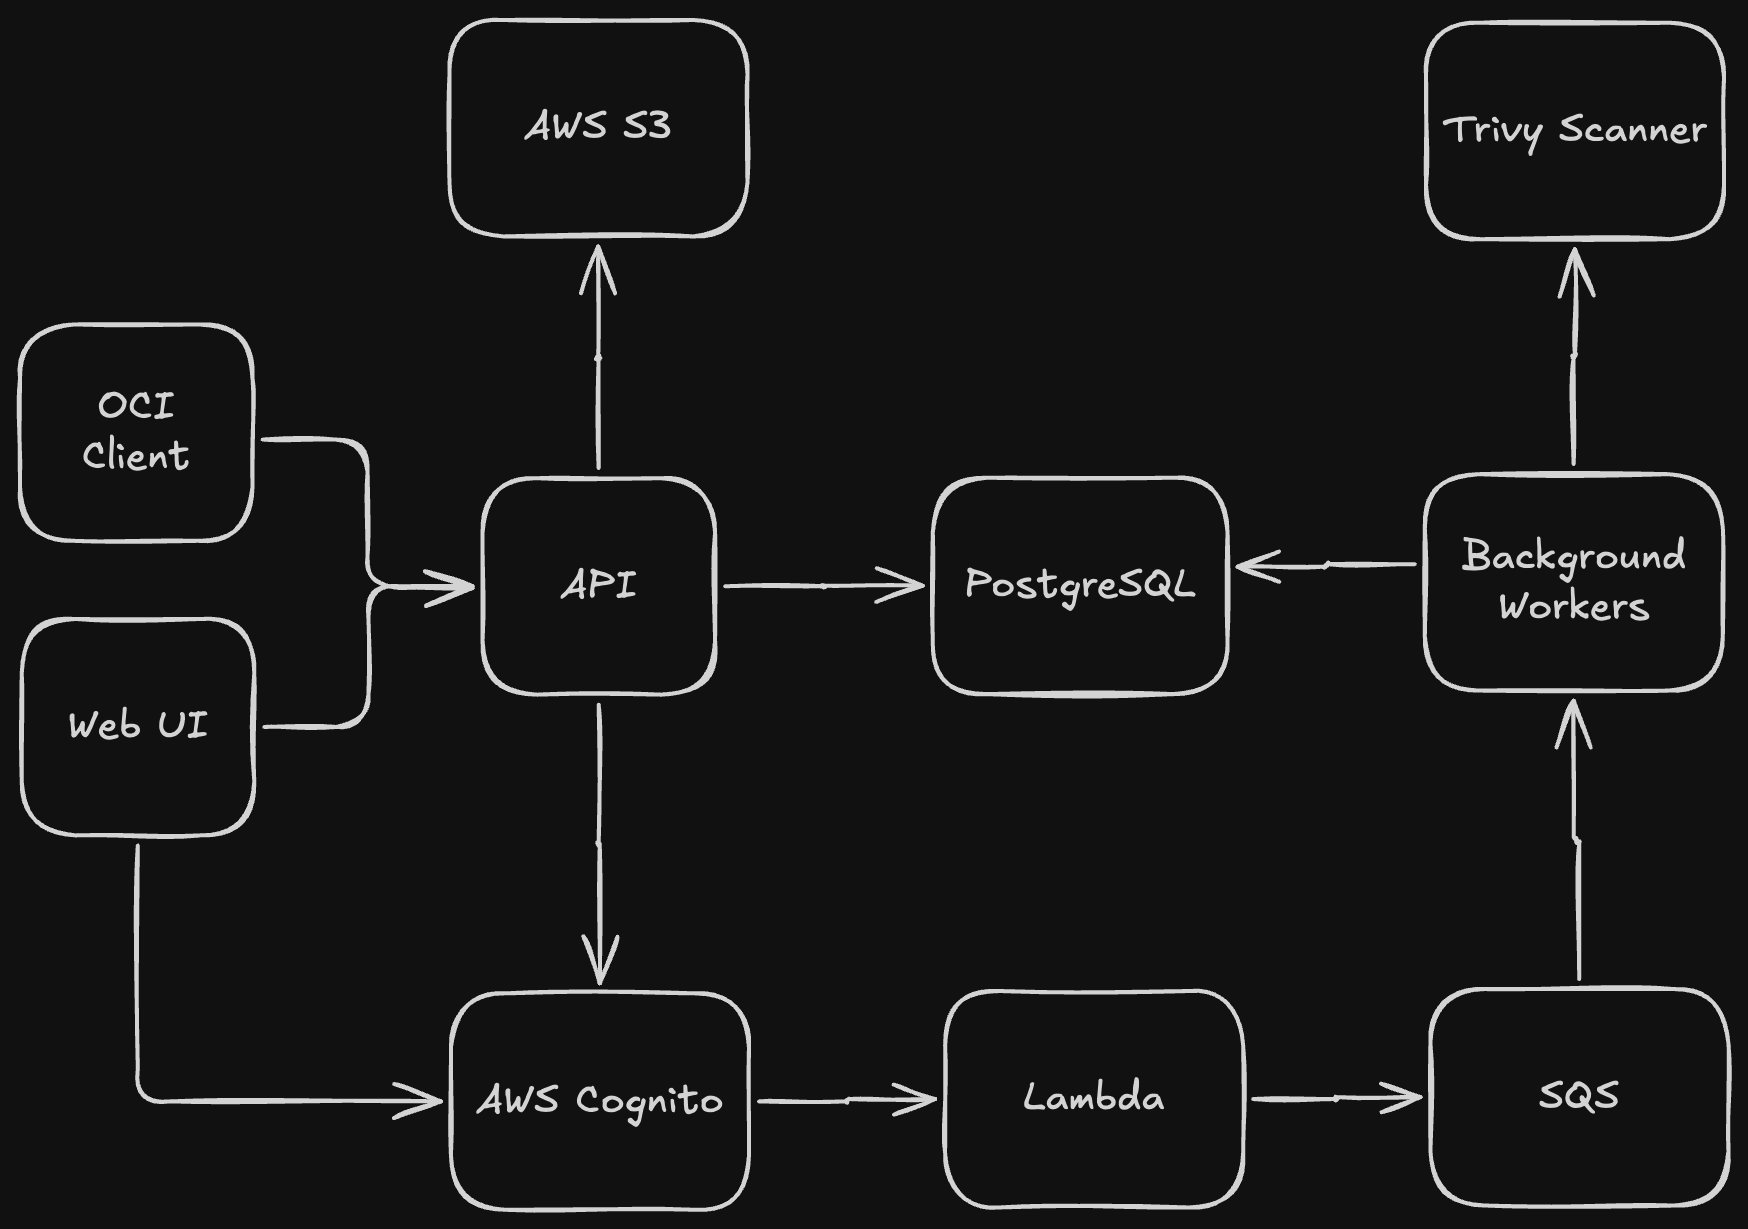
\includegraphics[scale=0.25]{architecture.png}

  \subsection{Technology Stack}

  For my tech stack I've selected the following:
  \begin{enumerate}
    \item GoLang[34] for Backend APIs
    \item PostgreSQL[35] for Database Engine
    \item NextJS[36] for Web UI Framework
    \item AWS S3 as storage layer
    \item AWS Cognito as OAuth2 Provider
    \item Trivy Scanner for vulnerability scanning
    \item Terraform[37] for Infrastructure as Code
    \item Terraform Cloud for orchestrating the deployment of AWS infrastructure
  \end{enumerate}

  I selected Golang as the main programing language for the backend API for the following reasons:

  \begin{itemize}
    \item Performance: Golang is a compiled language, offering high performance and low latency, which I think is critical for handling a large volume of artifact storage oeprations.
    \item Concurrency: It has built-in support for concurrency through goroutines, making it perfect for handling multiple simultaneous requests without the need for an external webserver.
    \item Ecosystem: The OCI ecosystem and related libraries are mostly implemented in golang, making it easier for my project to include them as dependencies if needed
    \item Simplicity: I find its syntax clean and easy to read, write and maintain
  \end{itemize}

  NextJS is a React-based framework with support for Server-side rendering, I selected this framework due to my familiarity with React thanks to the CM3050 Mobile Development module, and because its server-side rendering allows me to build a more secure WebUI, any sensitive data can be handled server-side and won't leak to the client unneccesarly. This also makes the frontend much more performant as complicated React components can be rendered on a server with more resources.

  \subsection{Repository Pattern}

  In the golang application I will be using the EntGO[38] entity framework. This is a simple ORM for querying a database and mapping data to Golang Structs.

  Keeping application along with database logic makes applications more complex, hard to test and maintain. So to avoid this I will be using the Repository Pattern to query the database.

  The repository pattern is a way to abstract the data layer, a repository acts as a middle layer between application logic and the data mapping layers, in EntGo the data mapping layer would be the Entity Schema.

  Each Database Schema model will have its own repository used by the application to CRUD information from the database. 

  Each API Endpoint Group will have its own Handler Struct, using dependency injection it will include dependencies to all the different repository structs it needs for the application logic to work.

  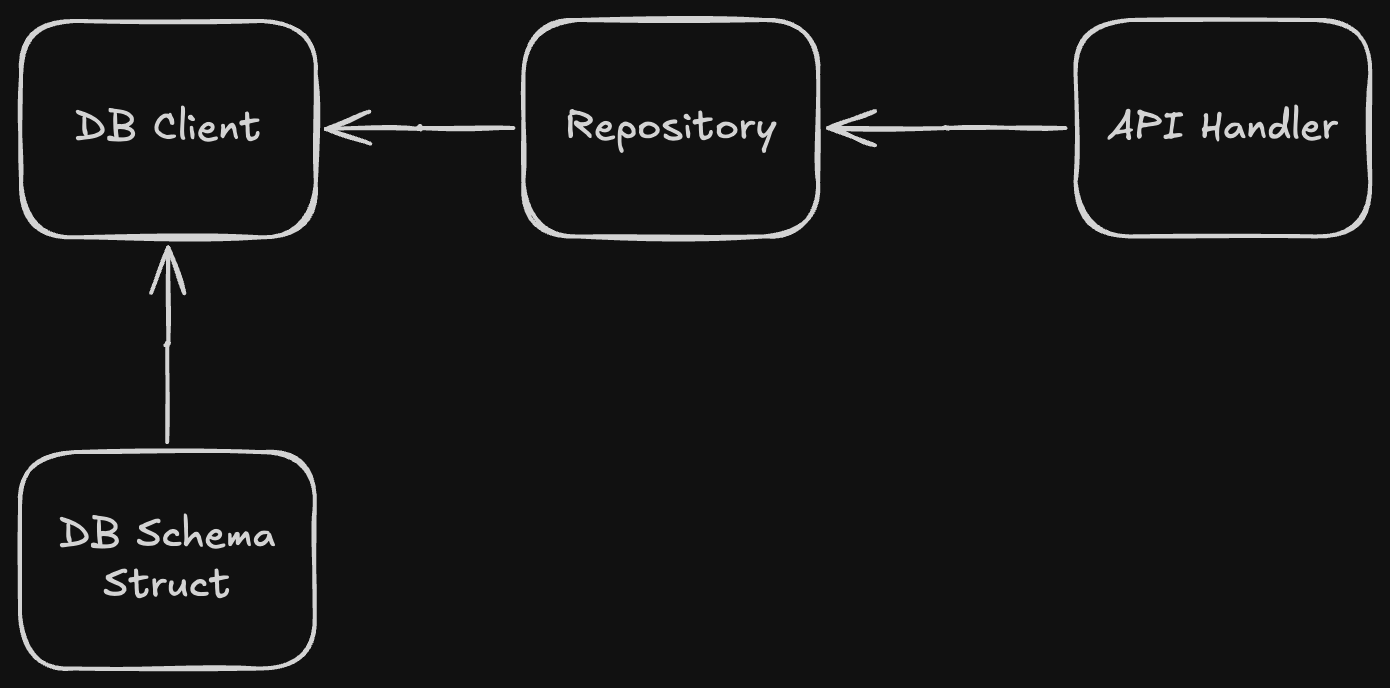
\includegraphics[scale=0.30]{repository_pattern.png}

  \subsection{Software Development Lifecycle}
  I'll be using Github as a Version Control system, I will have 3 different projects.

  \begin{enumerate}
    \item Backend API Source Code
    \item Web UI Source Code
    \item Terraform Code
  \end{enumerate}

  All changes to the 3 different projects will be submitted via the PR system in Github, this will allow for cleaner commit history and traceability of changes, and it will be paired with a CircleCI pipeline that will automatically execute any unit tests available and block the change to be merged if they fail.
  
  For organising work tasks I'm going to use Trello. I will be doing 1-week sprints, keeping them short will allow me to better plan work and break down stores to simpler tasks that can fit in one week.

  At the end of each sprint I will do a review of all the commited work, test each feature individually, create stories for Bugs if any are found and plan the next sprint.

  As I'm the only developer involved in the development it will be very hard to not be baised on all the submitted changes, to try to mitigate this I'm going to be leaning on the tooling provided by the go language to lint the code and perform static analysis of the changes. This will be included in the CircleCI pipeline and block me from merging changes if I don't solve the outstanding issues.

  \subsection{Testing the project}

  I will be testing my project in 3 different ways.

  Being fully OCI-compliant is the backbone of my idea, without being comformant with the specification I won't be able to develop the other features that depend on it. The OpenContainer Initiative provides an automated test suite[39] that developers can use to understand how compliant their projects are with the distribution specification, and outputs an HTML report. I will be using this test suite to identify gaps and issues on my OCI interface.

  I will be creating unit tests for all the developed APIs on the backend to validate each individual component in it. A CircleCI project will be used to automate running these tests on each commited change, this will ensure that new changes don't break existing functionality.

  Finally I will be doing some usability testing with some of my target users to evaluate the UX and interface design, the feedback gathered will be used to fix bugs and improve the different features.

  To test e2e functionality from a user perspective I will be using:

  \begin{itemize}
    \item Docker CLI
    \item ORAS CLI
    \item Helm v3 CLI
    \item Twine for upload of python packages
    \item PIP for installing python packages
  \end{itemize}
  

  \subsection{Gantt Chart}
  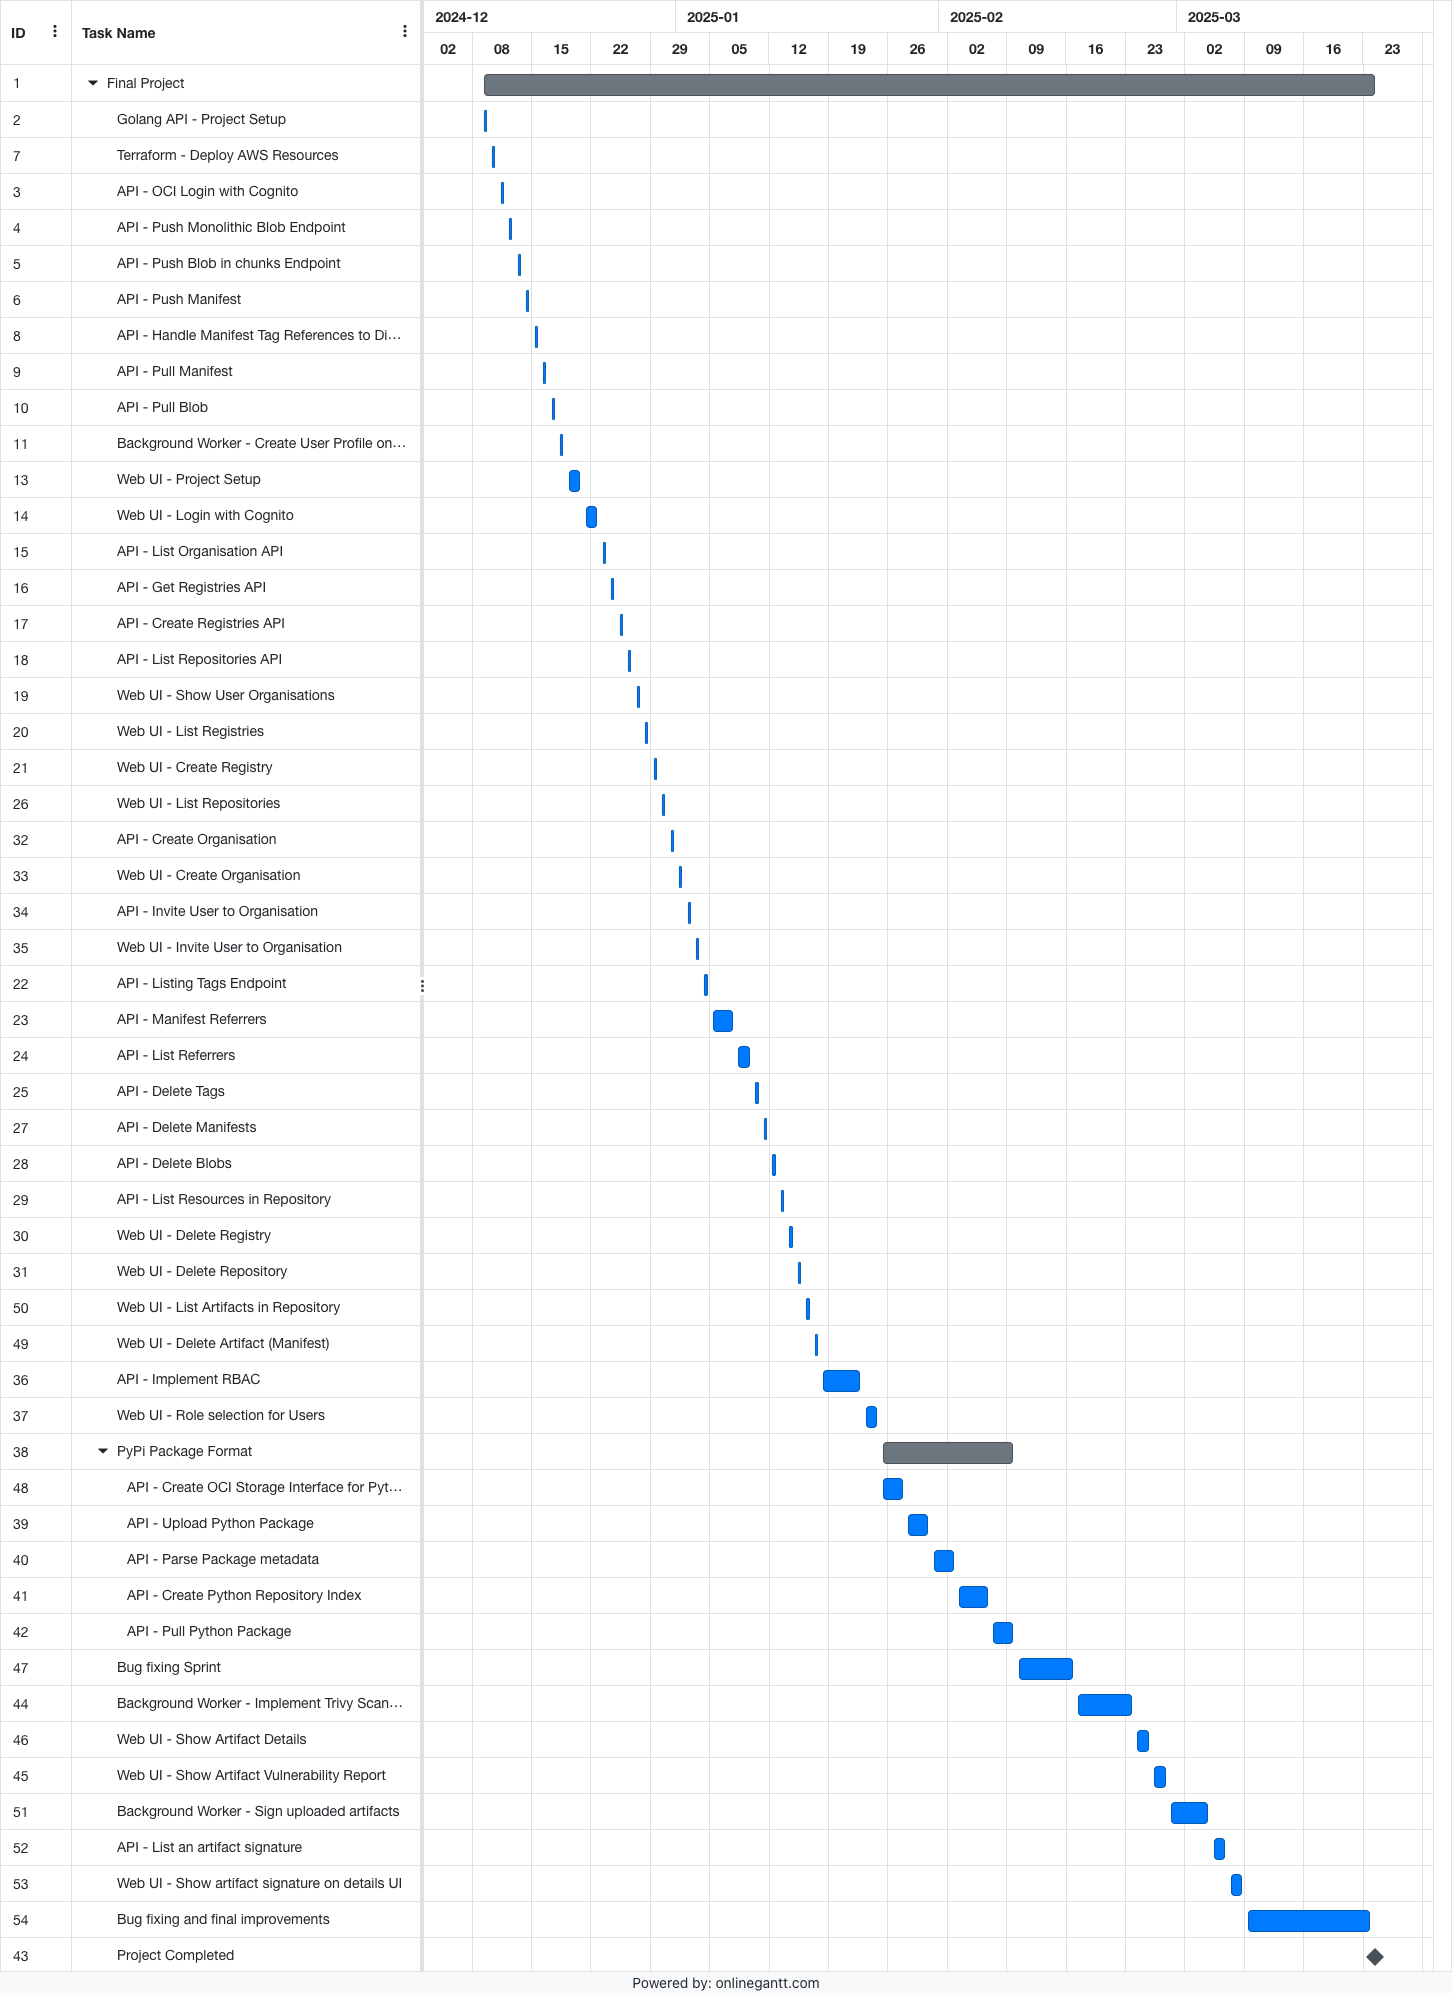
\includegraphics[scale=0.27]{gantt.png}

  \section{Prototype}

  \subsection{Backend API}

  My current prototype focuses on the following features of the backend:

  \begin{itemize}
    \item User login with AWS Cognito via OCI-tools
    \item Verifying the JWT token is valid on the backend
    \item Push Blobs (both in chunks and monolithically)
    \item Push Manifests
    \item Storing both Blobs and manifests on S3
    \item Referencing manifests with tags
    \item Pull Manifests
    \item Pull Blobs
    \item Background worker consume from SQS and create a starting Organisation on User signup
    \item Create Registry API Endpoint
    \item List Registries API Endpoint
    \item List Organisations API Endpoint
    \item List Repositories API Endpoint 
  \end{itemize}

  These features don't make the project OCI-compliant yet, but gives me the most basic actions to be able to test and evaluate the feasability of the upcoming work.

  Not all features are fully fledged out yet though, pushing manifests work as expected but I'm basically proxying the JSON through straight to storage without doing any validation of the document, a registry has to parse the manifest and check against the Image Specification[40] if its valid and if there are valid blobs in storage of each of the specified layers in it. This validation is currently lacking and it signifies a security risk as an attacker could push a manifest that points to layers not owned by them.

  I also had some issues with the web framework I selected, I initially started using the Gin Framework[41], but unfortunately it is very common for OCI artifacts to have forward slashes on their names, and they are used in the URL to query for information on them. Gin doesn't have good support for this, so I had to rewrite the backend in Chi[42].

  Chi is not a web framework but rather a composable router for building HTTP services, so it is less opinionaties and more flexible and allowed me to develop a custom URL matcher that I plugged into its HTTP router to support forward slashes as URL parameters.

  With all this I'm able to use the Docker CLI to login, pull and push images.

  \subsection{Web UI}

  The Web UI currently has the following features:
  \begin{itemize}
    \item WebUI can Signup and Login users via AWS Cognito
    \item A user can switch between organisation on the WebUI
    \item List of registries
    \item Create a registry
    \item List of repositories
  \end{itemize}

  To accelerate development, I'm using the free to use ShadCN UI[43] components.

  Current features are very basic as I've spent more time on backend development, I also underestimated the difficulty of building a website using NextJS and there was a learning curve that put me behind where I would like it to be at the time of writing this report. I'm hoping that now that I've learnt how to use it I can increase the development velocity of the UI once the more complicated features need to go in.

  \subsection{Screenshots}

  \subsubsection{Login and signup}

  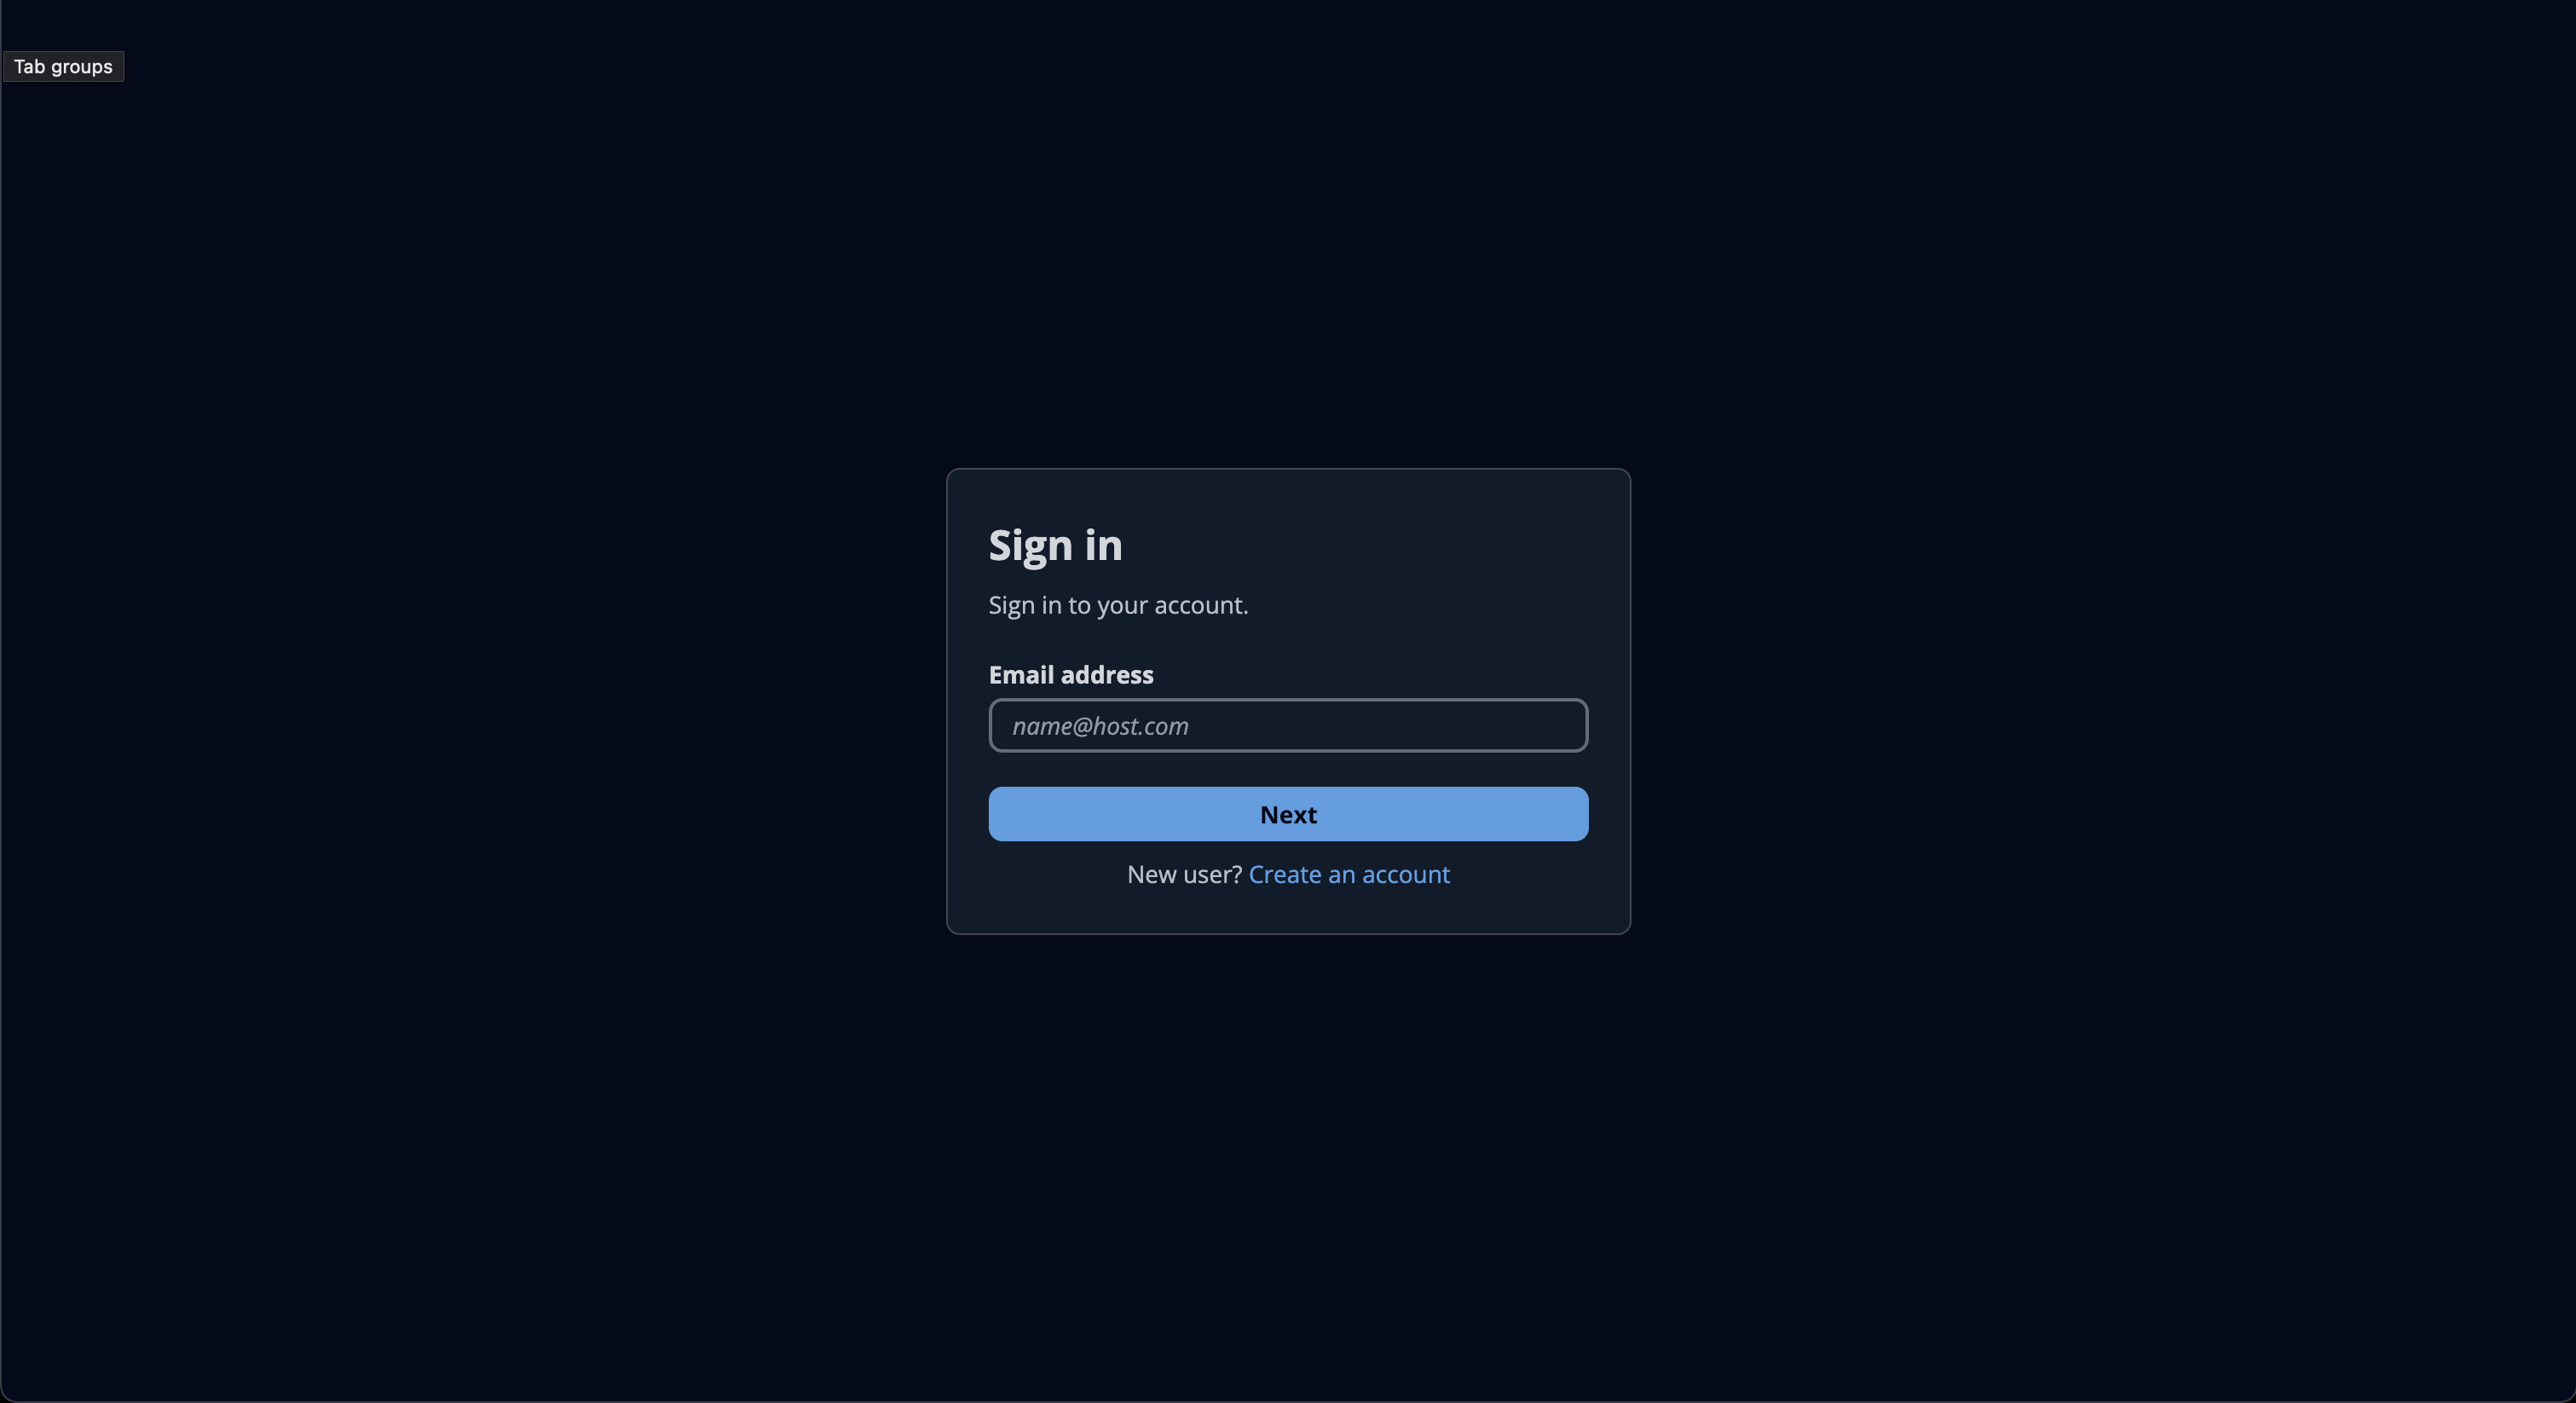
\includegraphics[scale=0.28]{screenshots/signin.png}

  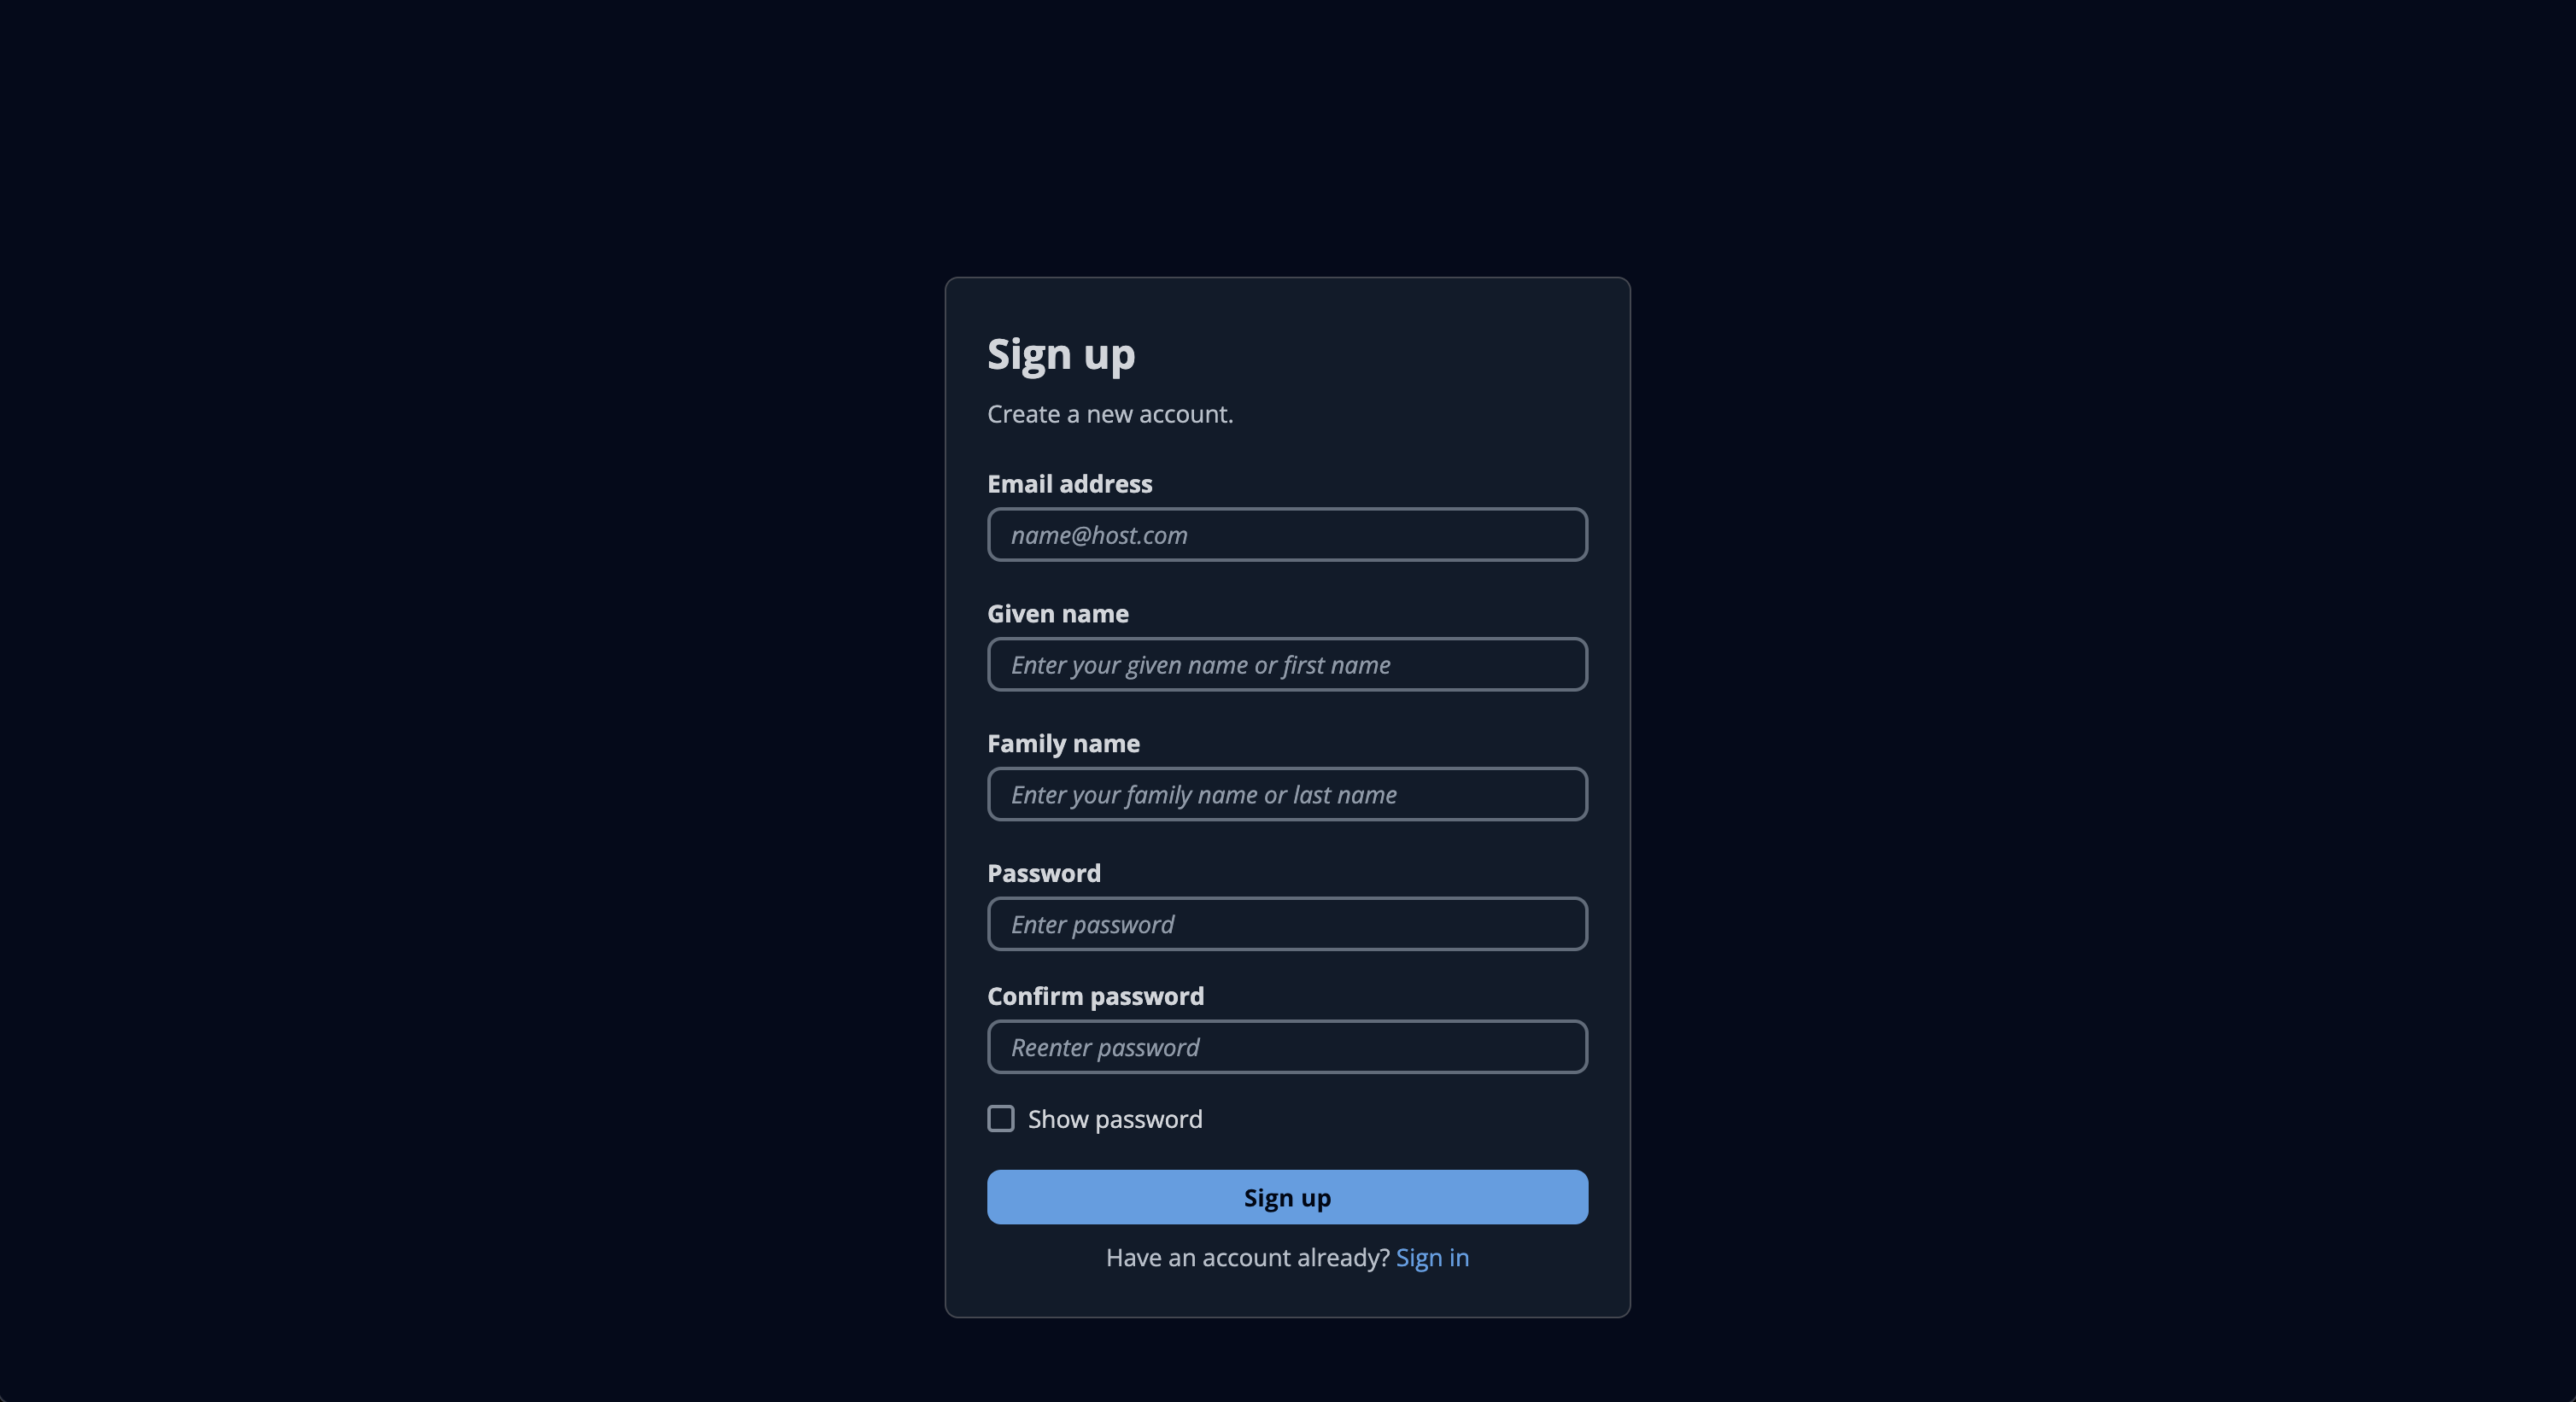
\includegraphics[scale=0.28]{screenshots/signup.png}

  \subsubsection{Dashboard}

  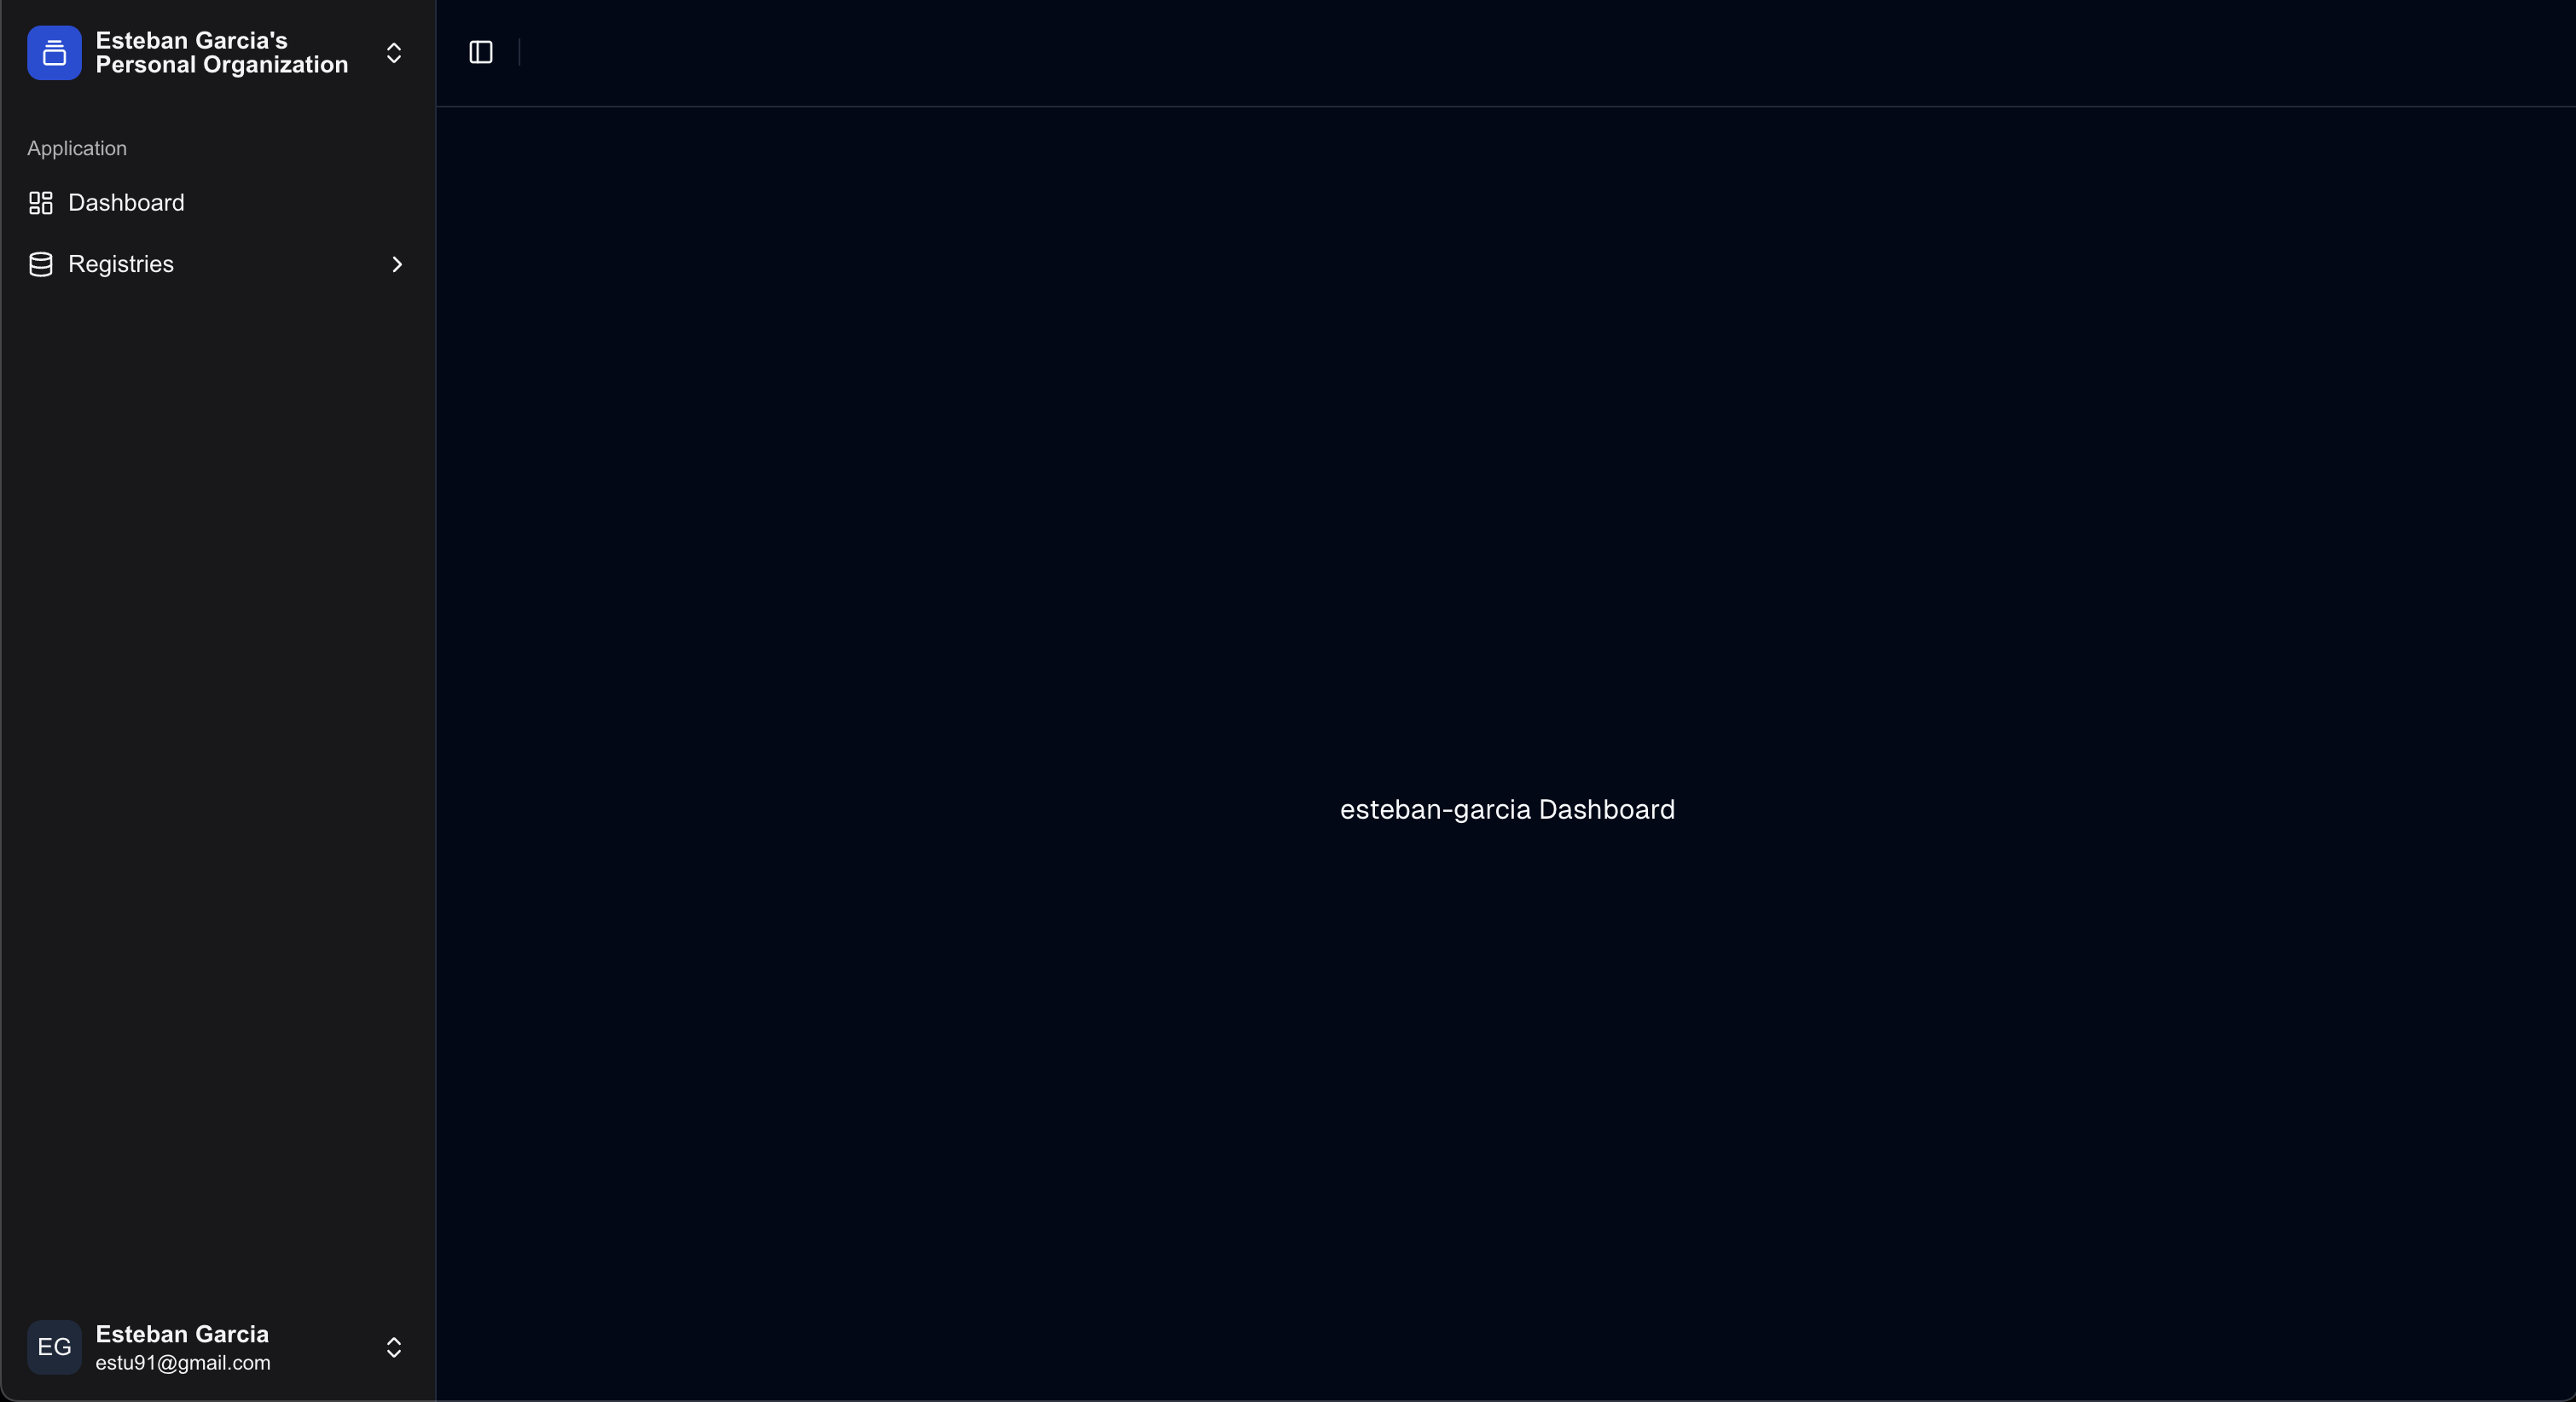
\includegraphics[scale=0.28]{screenshots/dashboard.png} 

  \subsubsection{Registries}

  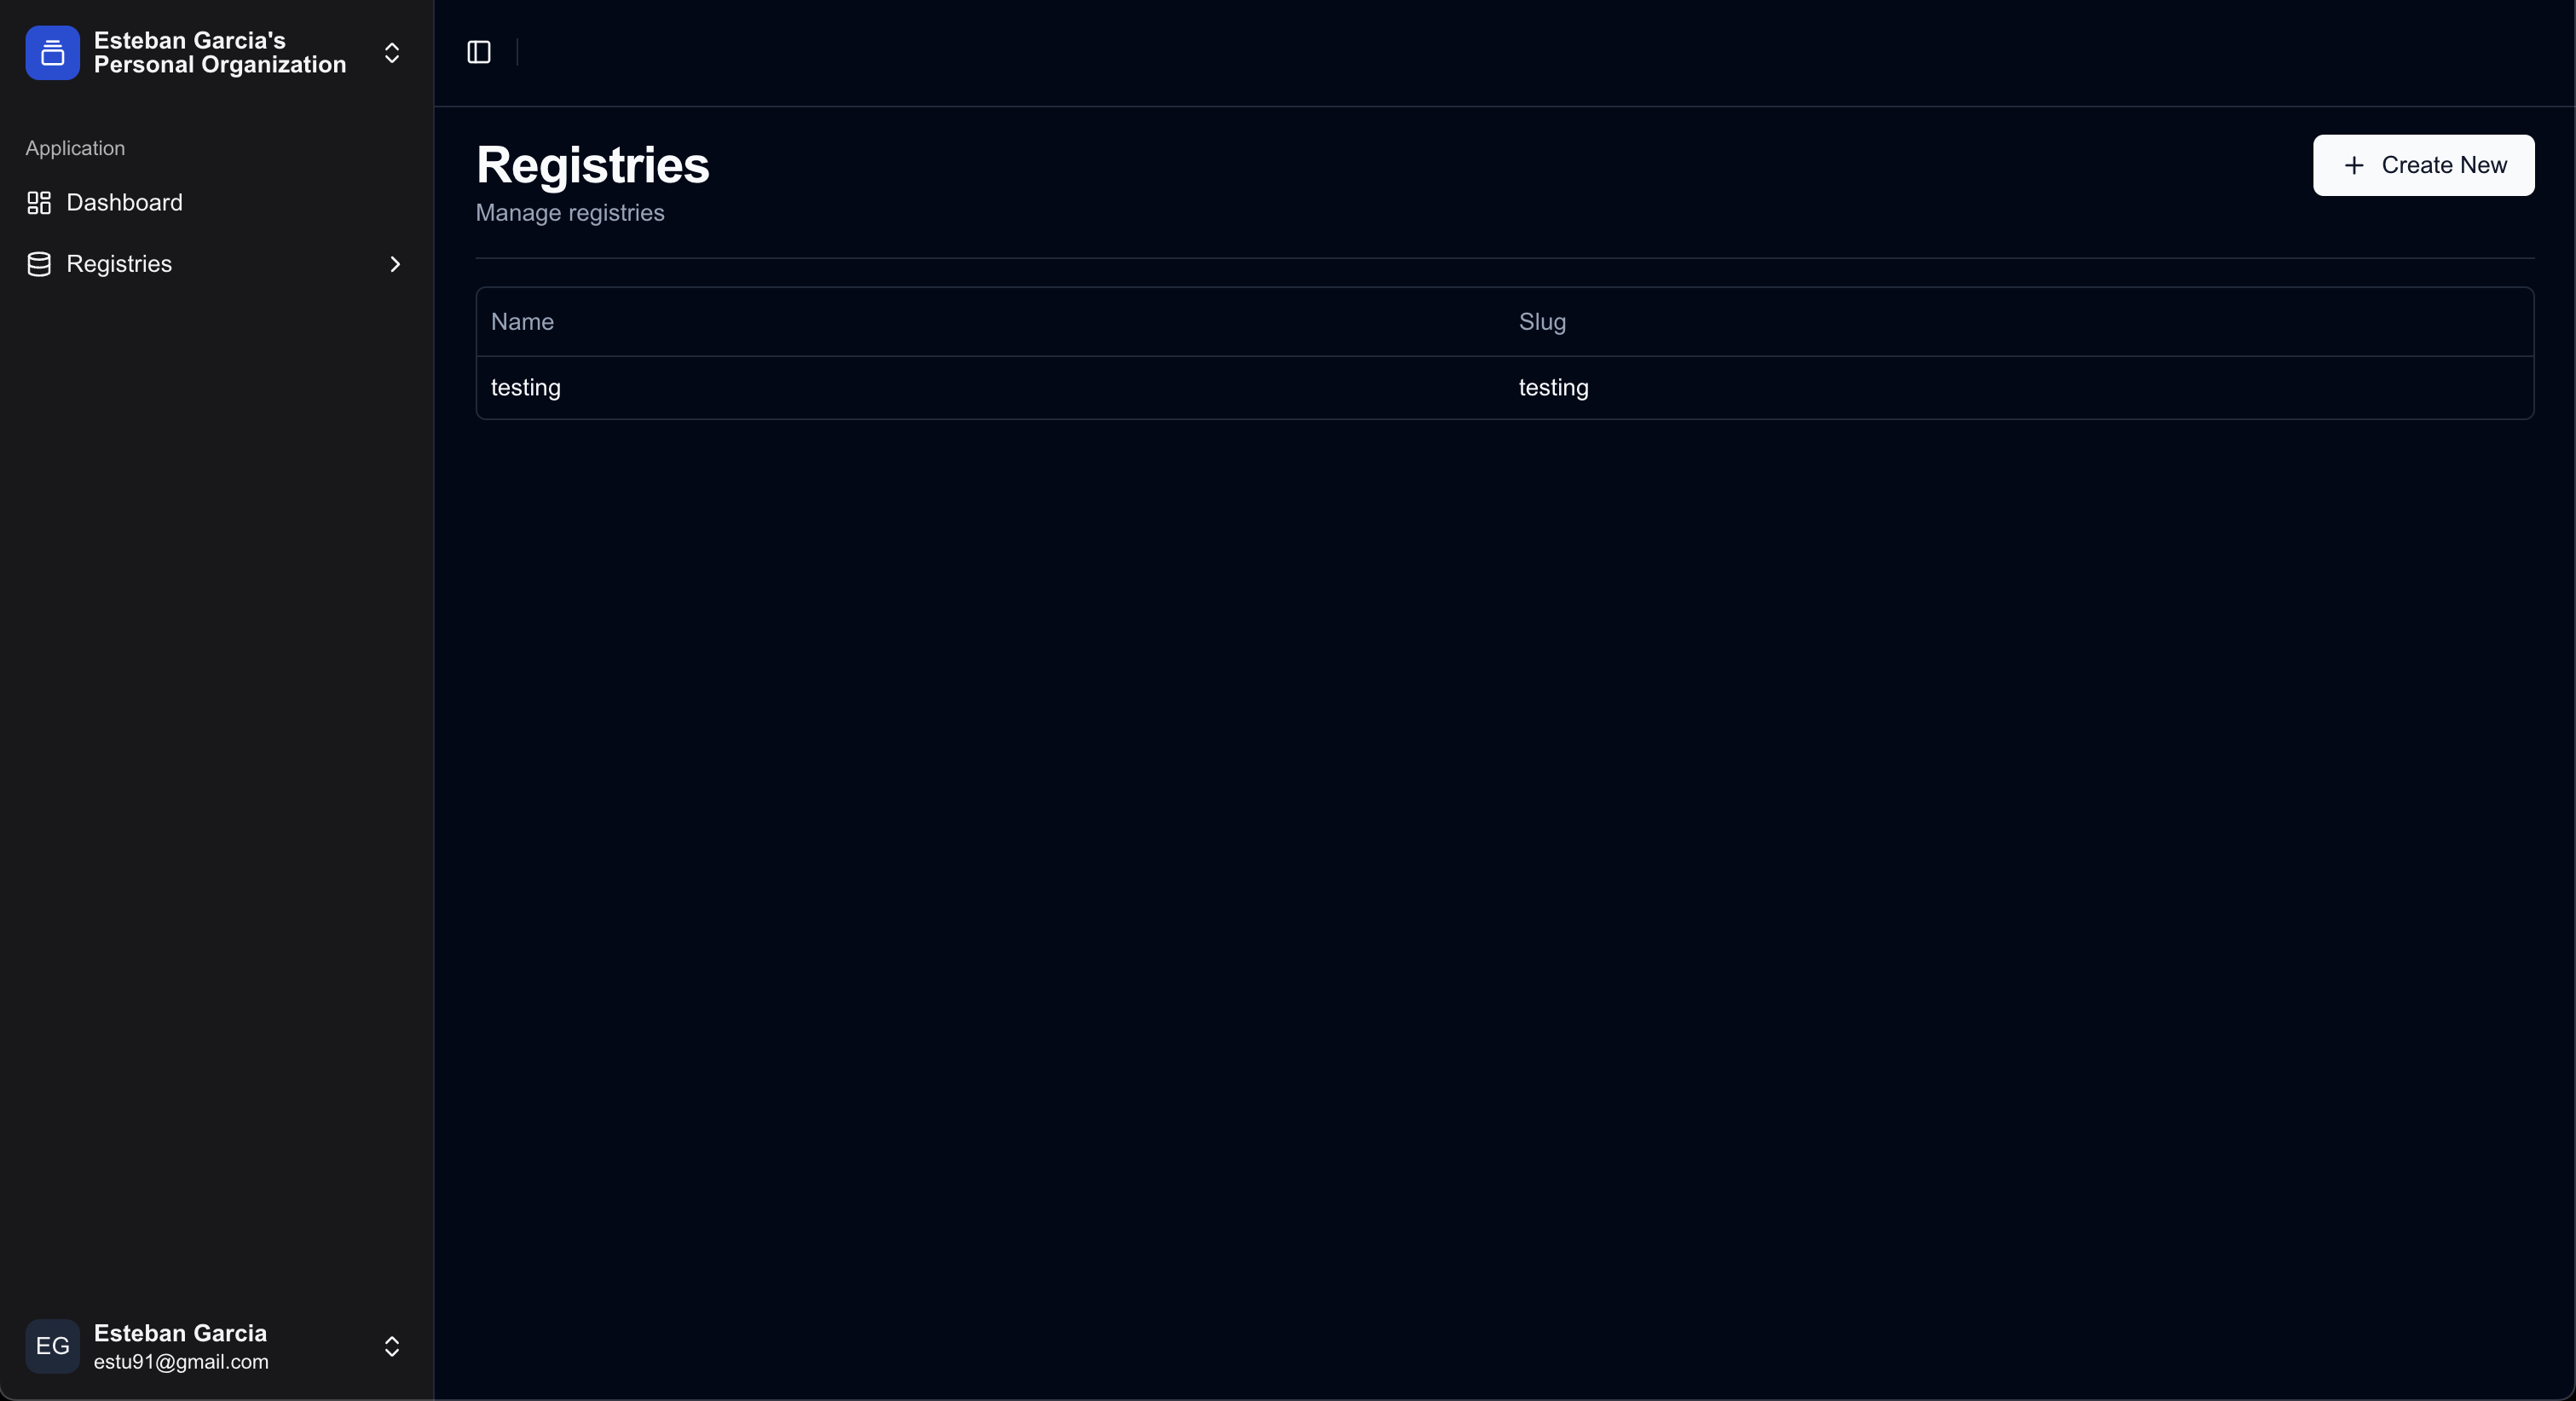
\includegraphics[scale=0.28]{screenshots/registries.png}

  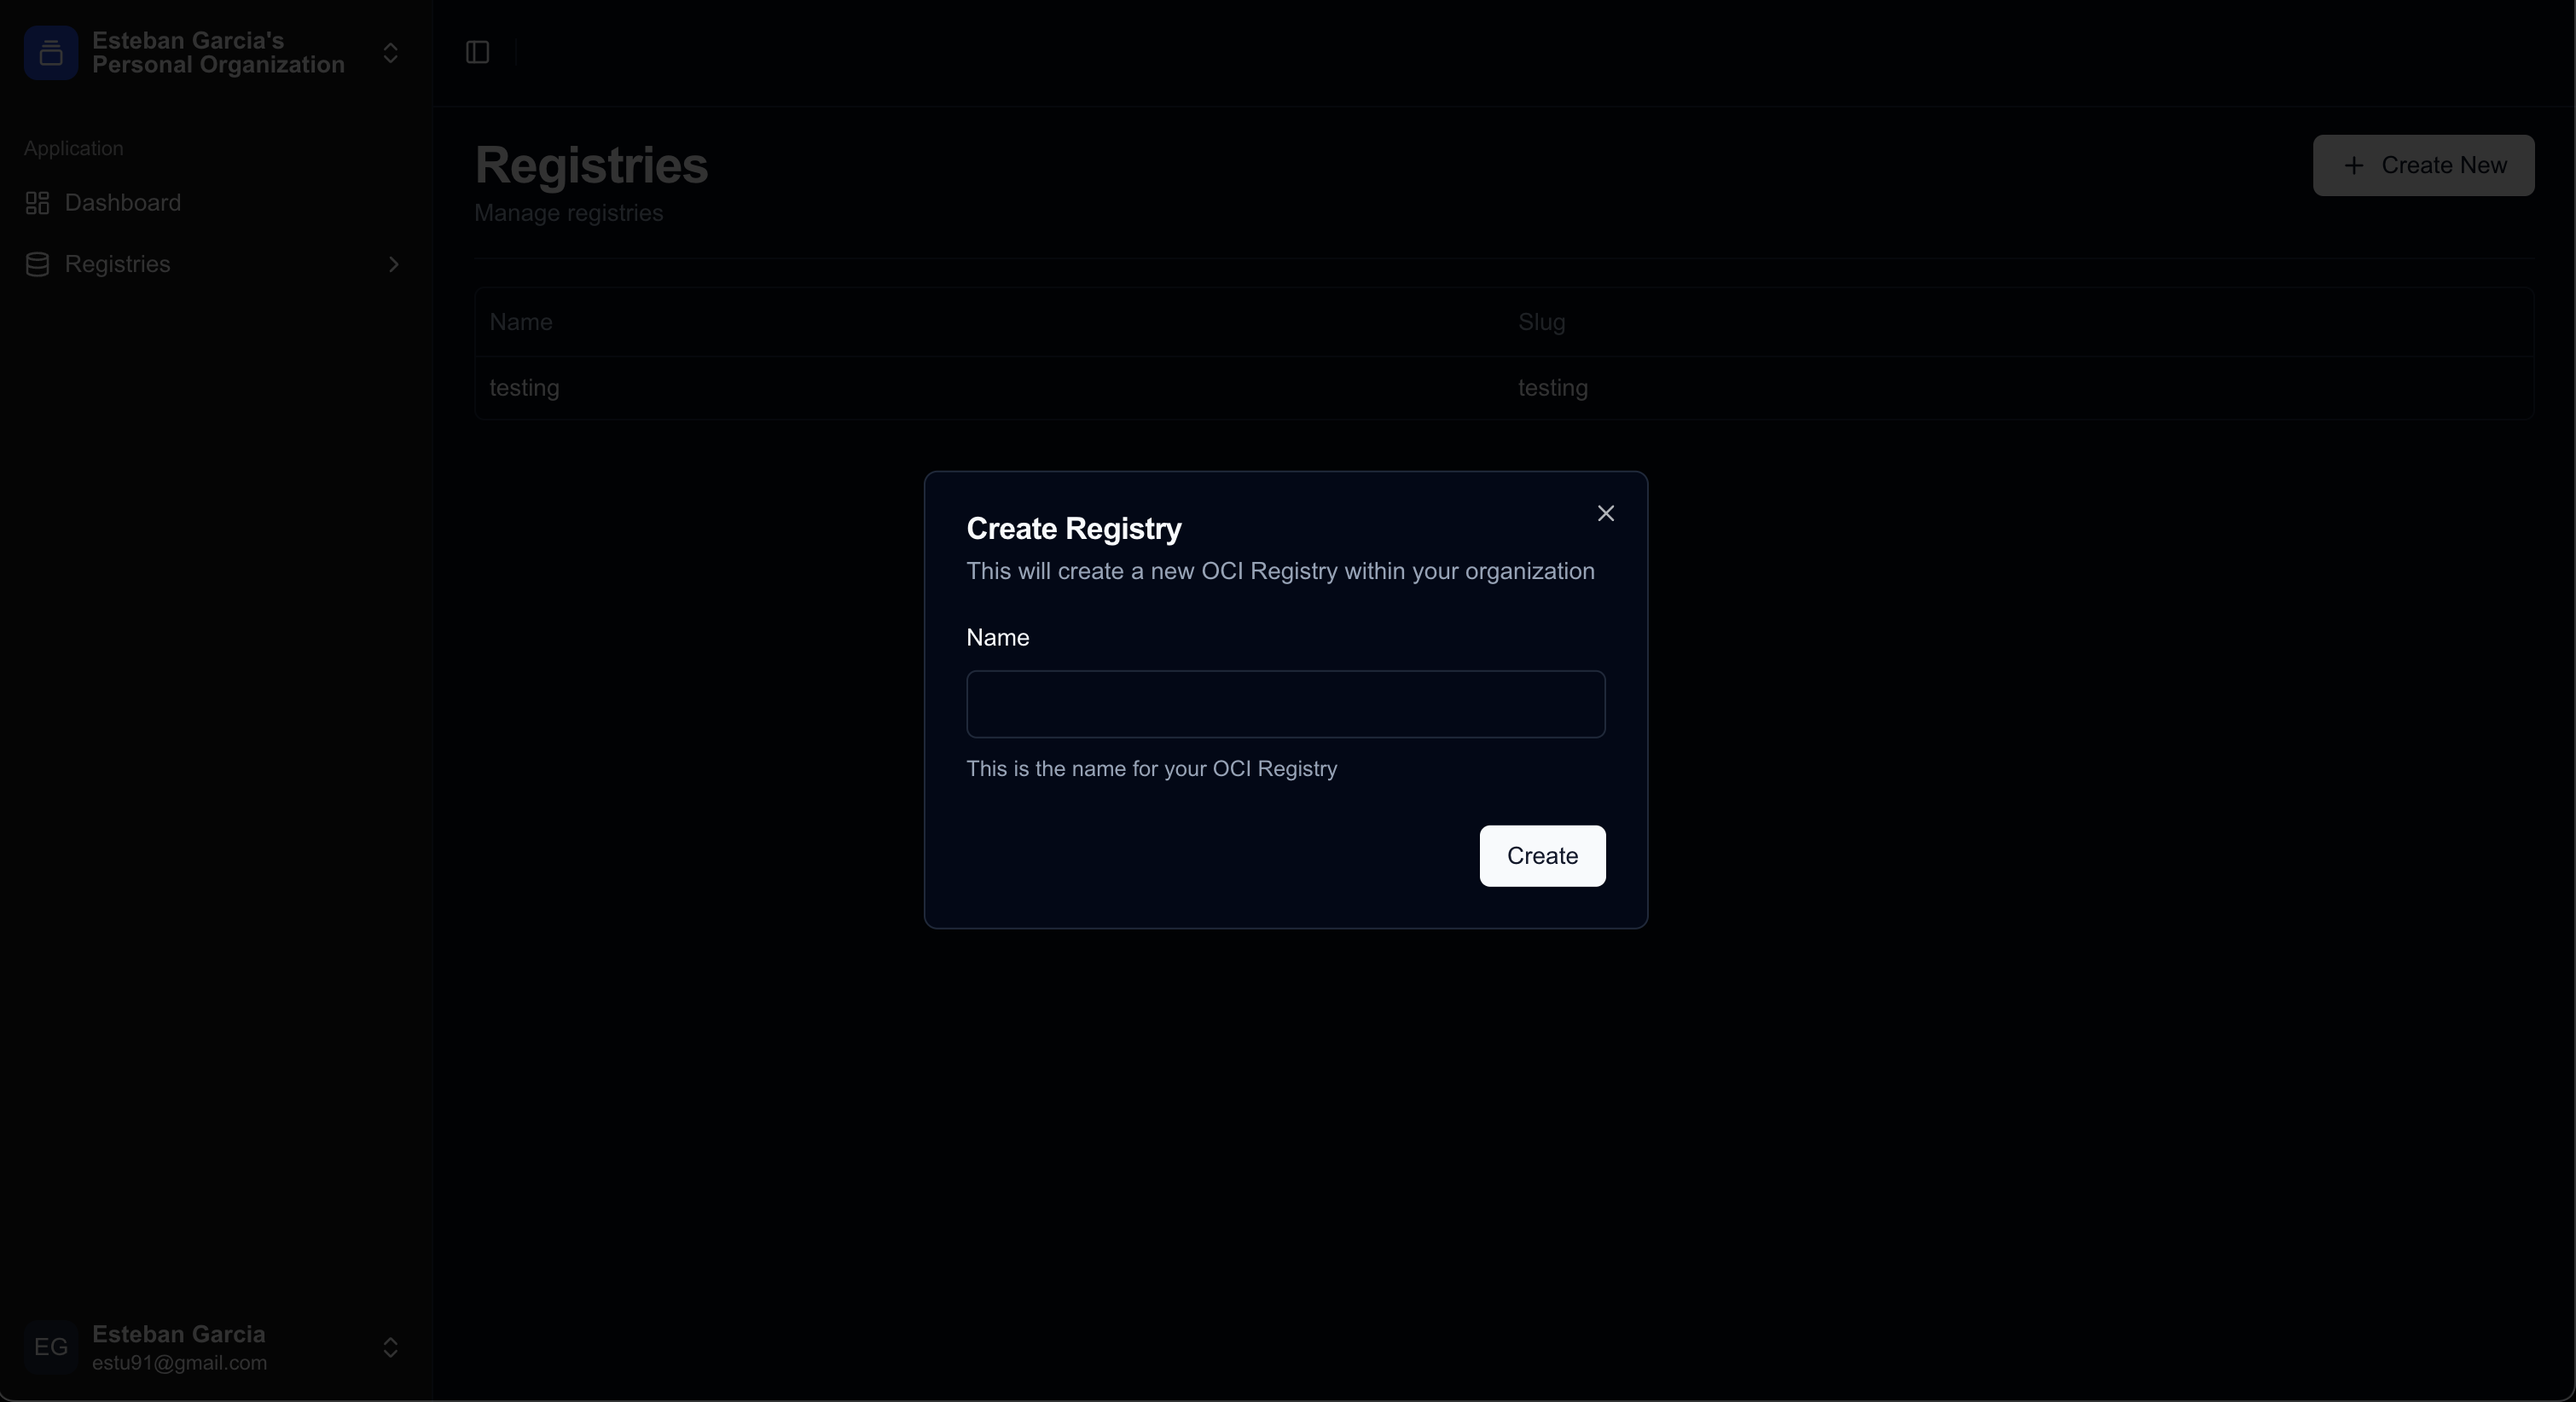
\includegraphics[scale=0.28]{screenshots/create-registry.png}

  \subsubsection{Repositories}

  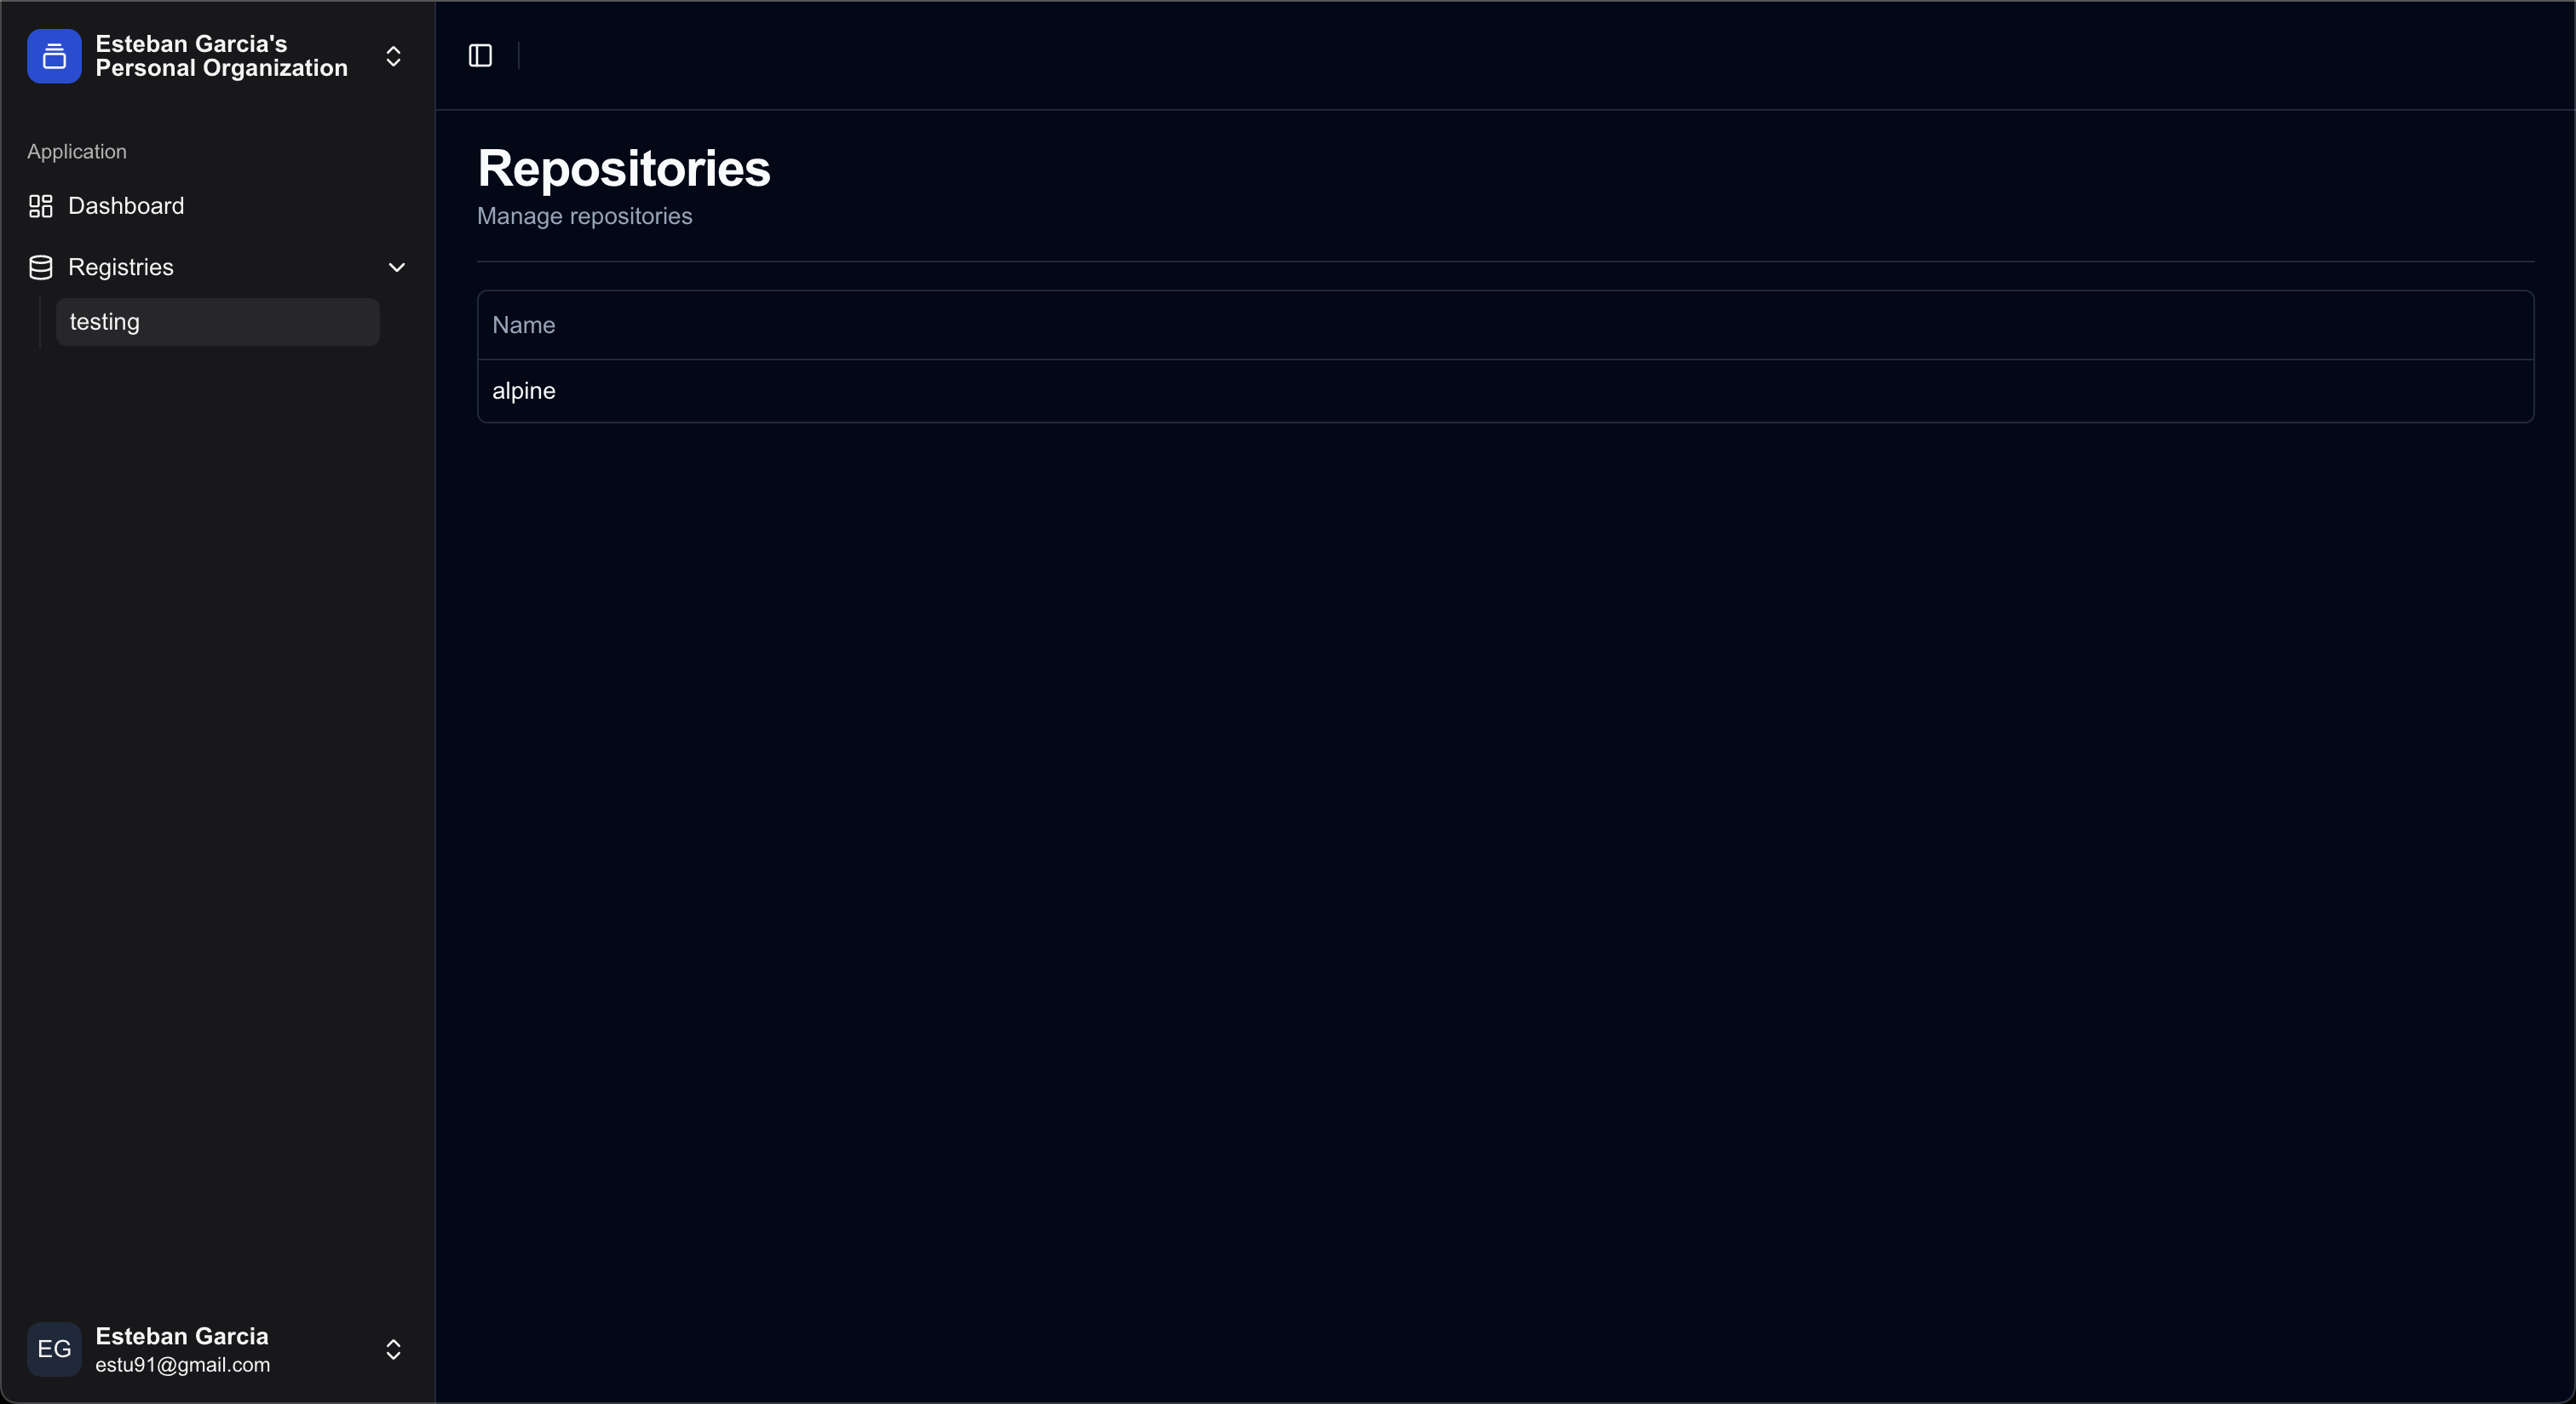
\includegraphics[scale=0.28]{screenshots/repositories.png}

  \newpage

  \section{References}

  [1] `OpenContainer Initiative', \url{https://opencontainers.org/}
  
  [2] `Docker Inc.', \url{https://docs.docker.com/get-started/docker-concepts/the-basics/what-is-an-image/}

  [3] `Helm', \url{https://helm.sh/docs/topics/charts/}

  [4] `PyPi', \url{https://pypi.org/}

  [5] `JFrog Artifactory', \url{https://jfrog.com/artifactory/}

  [6] `Harbor', \url{https://goharbor.io/}

  [7] `How Low Can You Go? An Analysis of 2023 Time-to-Exploit Trends', Casey Charrier; Robert Weiner, October 15, 2024, Google, \url{https://cloud.google.com/blog/topics/threat-intelligence/time-to-exploit-trends-2023}

  [8] `JFrog Xray', \url{https://jfrog.com/help/r/get-started-with-the-jfrog-platform/jfrog-xray}

  [9] `Security Keys Management', JFrog, July 2024, \url{https://jfrog.com/help/r/jfrog-platform-administration-documentation/security-keys-management}

  [10] `VMWare Inc.', \url{https://www.vmware.com/}

  [11] `Cloud Native Computing Foundation', \url{https://www.cncf.io/}

  [12] `Trivy Project', \url{https://github.com/aquasecurity/trivy}

  [13] `Clair Project', \url{https://github.com/quay/clair}
  
  [14] `Top Five Challenges in Software Supply Chain Security: Observations From 30 Industry and Government Organizations', William Enck;Laurie Williams, March 2022, \url{https://ieeexplore.ieee.org/abstract/document/9740718}

  [15] `Discord Token Stealer Discovered in PyPI Repository', Bertus, Jan 2019, \url{https://bertusk.medium.com/discord-token-stealer-discovered-in-pypi-repository-e65ed9c3de06}

  [16] `Securing the Software Supply Chain', NSA, August 2022, \url{https://media.defense.gov/2022/Sep/01/2003068942/-1/-1/0/ESF_SECURING_THE_SOFTWARE_SUPPLY_CHAIN_DEVELOPERS.PDF}

  [17] `Open Container Initiative Distribution Specification', Feb 2024, \url{https://github.com/opencontainers/distribution-spec/blob/v1.1.0/spec.md}

  [18] `POST followed by PUT Blob Upload', Feb 2024, \url{https://github.com/opencontainers/distribution-spec/blob/main/spec.md#post-then-put}

  [19] `Single POST Blob Upload', Feb 2024, \url{https://github.com/opencontainers/distribution-spec/blob/main/spec.md#single-post}

  [20] `Listing referrers', \url{https://github.com/opencontainers/distribution-spec/blob/main/spec.md#listing-referrers}

  [21] `ORAS Project', \url{http://oras.land}

  [22] `Twine', \url{https://pypi.org/project/twine/}
  
  [23] 'Bearer Authentication`, \url{https://swagger.io/docs/specification/v3_0/authentication/bearer-authentication/}

  [24] `JSON Web Tokens', \url{https://jwt.io/introduction}

  [25] `AWS Cognito', \url{https://docs.aws.amazon.com/cognito/}

  [26] `OAuth 2.0', \url{https://oauth.net/2/}

  [27] `Amazon Simple Storage Service', \url{https://docs.aws.amazon.com/s3/}

  [28] `Data Protection in S3', \url{https://docs.aws.amazon.com/AmazonS3/latest/userguide/DataDurability.html}

  [29] `Uploading and copying objects using multipart upload in Amazon S3', \url{https://docs.aws.amazon.com/AmazonS3/latest/userguide/mpuoverview.html}

  [30] `Sharing objects with presigned URLs', \url{https://docs.aws.amazon.com/AmazonS3/latest/userguide/ShareObjectPreSignedURL.html}

  [31] `PyPi Upload API', \url{https://docs.pypi.org/api/upload/}

  [32] `PEP-503 HTML', \url{https://peps.python.org/pep-0503/}

  [33] `PEP 691 – JSON-based Simple API for Python Package Indexes', \url{https://peps.python.org/pep-0691/}
  
  [34] `Go Programming Language', \url{https://go.dev/}

  [35] `PostgreSQL Database Engine', \url{https://www.postgresql.org/}

  [36] `NextJS Framework', \url{https://nextjs.org/}

  [37] `Terraform IaC', \url{https://www.terraform.io/}

  [38] `EntGo Entity Framework', \url{https://entgo.io/}

  [39] `OCI Conformance Tests', \url{https://github.com/opencontainers/distribution-spec/tree/main/conformance}

  [40] `OCI Image Manifest Specification', \url{https://github.com/opencontainers/image-spec/blob/main/manifest.md}

  [41] `Gin Web Framework', \url{https://github.com/gin-gonic/gin}

  [42] `Chi Router', \url{https://github.com/go-chi/chi}

  [43] `shadcn/ui', \url{https://ui.shadcn.com/}

\end{document}
